\documentclass[article]{jss}
%\usepackage{thumbpdf}
\usepackage{comment}

\author{Michael Lawrence\\
Iowa State University \And Duncan Temple Lang\\
University of California - Davis}

\title{\pkg{RGtk2}:\\A Graphical User Interface Toolkit for
\proglang{R}}

\Plainauthor{Michael Lawrence, Duncan Temple Lang}
\Plaintitle{RGtk2: A Graphical User Interface Toolkit for R} 
\Shorttitle{RGtk2} 

\Abstract{
Graphical User Interfaces (GUIs) are growing in popularity as a
complement or alternative to
the traditional Command Line Interfaces (CLIs) to \proglang{R}.
\pkg{RGtk2} is an 
\proglang{R} package for creating \proglang{R} GUIs. The package
provides programmatic access
to \pkg{GTK+} 2.0, an open-source GUI toolkit written in \proglang{C}.
To 
construct a GUI, the \proglang{R} programmer calls \pkg{RGtk2}
functions that
map to functions in the underlying \pkg{GTK+} library. This paper
introduces
the basic concepts underlying \pkg{GTK+} and explains how to use
\pkg{RGtk2}
to construct GUIs from \proglang{R}. The tutorial is based on simple
and
pratical programming examples. We also provide more complex examples 
illustrating the advanced features of the package. The design of the
\pkg{RGtk2} API and the
low-level interface from \proglang{R} to \pkg{GTK+} are discussed at
length.
We compare \pkg{RGtk2} to alternative GUI toolkits for \proglang{R}. 
The package is available from CRAN.
}

\Keywords{graphical user interface, GUI, R, GTK+}

\Address{Michael Lawrence\\
Department of Statistics\\
Iowa State University\\
Ames, IA, USA\\
E-mail: lawremi@iastate.edu\\
}

\begin{document}

\section{Introduction}

% General

% interfaces
An interface, in the most general sense, is the boundary across which
two
entities communicate. In most cases, the communication is
bidirectional, 
involving input and output from both of the interfaced entities. In
computing,
there are two general types of interfaces: machine interfaces and user
interfaces
\citep{gui-cli}. A machine interface does not involve humans, while a 
user interface is between a human and a machine. In this paper, the
machines of
interest are software, and the central software component is the
\pkg{R} 
platform and language for statistical computing \citep{R}.

% user interfaces
Two common types of user interfaces in statistical computing are the
Command
Line Interface (CLI) and the Graphical User Interface (GUI). The usual
CLI 
consists of a textual console where the user types a sequence of
commands
at a prompt. The \proglang{R} console is an example of a CLI. The GUI
is the primary
means of interacting with desktops, like Windows and Mac OS, and
statistical software like JMP \citep{JMP}. These
interfaces are based on the WIMP (Window, Icon, Menu and Pointer)
paradigm 
\citep{WIMP}. WIMP was developed at Xerox PARC in the 1970's and was
popularized by 
the Apple Macintosh. On a WIMP desktop, application GUIs are contained
within 
windows, and resources, such as documents, are represented by
graphical icons. 
User actions are packed into hierarchical drop-down menus. The user
manipulates
the windows, icons and menus with a pointer device, such as a mouse.
The windows,
icons, and menus, as well as other graphical controls such as buttons,
sliders and 
text fields, have come to be known as \emph{widgets}. The graphical
nature and 
overall complexity of widgets makes their implementation a non-trivial
task.  
To alleviate the burden on the application
programmer, reusable widgets are collected into \emph{widget
toolkits}.

% motivation for guis
There is often debate over the relative merits of a CLI and a GUI
lacking a console. The comparison largely depends on the skills and
needs of the user \citep{gui-cli}. Effective use of a CLI requires the
user to be proficient in the command language understood by the
interface. For example, with a CLI, \pkg{R} users need to understand
the \proglang{R} language. Learning a computer language often demands
a significant commitment of time and energy; however, given a
small amount of knowledge, one can use the language to perform
arbitrary, rich tasks.  A graphical interface is much less general
and restrictive, but typically makes performing a specific task
easier. It does this two different ways: a) stream-lining the steps
involved in the task by providing a constrained context, and b)
removing the need to remember function names and syntax.  Different
users benefit from the two different interfaces for different tasks. 
And there is little doubt that for occasional users of a language and
for users focused a specific task, a GUI is easier to learn and more
accessible than a general purpose programming language.

% GUIs for R
Considering the widespread use and popular appeal of the \pkg{R}
platform and the rich set of state-of-the-art statistical methodology
it provides, it is desirable to try to make these available to a
broader set of users by simplifying the knowledge needed to use such
methods.
%DTL: importance is not an absolute thing, but a subjective decision
%and making R accessible to as many users is only importance if world
%domination is the goal.  For better science, it is not the number but
%the quality of users. For many, R is not the right thing - with or
%without a GUI.
The CLI has always been the most popular interface to \proglang{R} as
it is the generic interface provided on all platforms and there has
been much less focus in the R community on providing graphical
interfaces for specific tasks.  On some platforms, a CLI is a
component of a larger GUI with menus containing various utilities for
working with \proglang{R}. Examples of CLI-based \proglang{R} GUIs
include the official Windows and Mac OS X GUIs, as well as the
cross-platform Java GUI for R (JGR) \citep{JGR}. Although these
interfaces are GUIs, they are still very much in essence CLIs, in that
the primary mode of interacting with \proglang{R} is the same. Thus,
these GUIs appeal mostly to the power users of \proglang{R}.  A
separate set of GUIs targets the second group of users, those learning
the \proglang{R} language. Since this group includes many students,
these GUIs are often designed to teach general statistical concepts in
addition to \proglang{R}.  A CLI component is usually present in the
interface, though it is deemphasized by the surrounding GUI, which is
analogous to a set of ``training wheels'' on a bicycle. Examples of
these GUIs include Poor Man's GUI (pmg) \citep{pmg} and R Commander
\citep{rcmndr}. The third group of users, those who only require
\proglang{R} for certain tasks and do not wish to learn the language,
are targeted by task-specific GUIs. These interfaces usually do not
contain a command line, as the limited scope of the task does not
require it. If a task-specific GUI fits a task particularly well, it
may even appeal to an experienced user. There are many examples of
task-specific GUIs in \proglang{R}, including exploRase
\citep{explorase}, limmaGUI \citep{limma} and Rattle \citep{rattle}.

% GUIs in R
The task-specific GUIs, as well as more general \proglang{R} GUIs,
are often implemented in the \proglang{R} language. The main advantage
to 
writing a GUI in \proglang{R} is direct access to its statistical
analysis
functionality. The extensible nature of the \proglang{R} language and
its support 
for rapid prototyping particularly faciliate the construction of
task-specific GUIs.
Building a GUI in \proglang{R}, as in any language, is made easier
through the use of a 
widget toolkit. The \pkg{tcltk} package \citep{Rnews:Dalgaard:2001a,
Rnews:Dalgaard:2002},
which provides access to \pkg{tcl/tk} \citep{ousterhout,welch}, is the
most often 
used GUI toolkit for \proglang{R}. Others include \pkg{RGtk}
\citep{RGtk}, based
on \pkg{GTK+} \citep{GTK}; \pkg{RwxWidgets} \citep{RwxWidgets}, based
on
wxWidgets \citep{wxwidgets}; and \pkg{gWidgets} \citep{gWidgets}, a
simplified, common interface to several toolkits, including
\pkg{GTK+}, \pkg{tcl/tk}
and \proglang{Java} \pkg{Swing}. There are also packages for embedding
\proglang{R}
graphics in custom interfaces, such as \pkg{gtkDevice}
\citep{gtkDevice} 
and \pkg{cairoDevice} \citep{cairoDevice} for \pkg{GTK+} and
\pkg{tkrplot} 
\citep{tkrplot} for \pkg{tcl/tk}.

% RGtk2
\pkg{RGtk2} is a GUI toolkit for \proglang{R} derived from the
\pkg{RGtk} package.
Like \pkg{RGtk}, \pkg{RGtk2} provides programmatic access to
\pkg{GTK+}, 
a cross-platform (Windows, Mac, and Linux) widget toolkit. 
% DTL: already cited \citep{GTK}.
The letters \emph{GTK} stand for the \emph{GIMP ToolKit}, with the
word \emph{GIMP} recording the origin of the library as part of the
GNU Image Manipulation Program. \pkg{GTK+} is written in \proglang{C},
which
facilitates access from languages like \proglang{R} that are also
implemented 
in \proglang{C}. It is licensed under the \emph{Lesser GNU Public
License} (LGPL),
%DTL:  meaning that \pkg{GTK+} does not force a specific license on
%the software that uses it.
% Yes it does. It forces the LGPL by definition
which provides greater flexibility and more wide-spread use than the
regular GPL license.
This contributes to its popularity. \pkg{GTK+} provides the same
widgets 
on every platform, though it can be customized to emulate 
platform-specific look and feel. The original \pkg{RGtk} is bound to
the previous
generation of \pkg{GTK+}, version 1.2. \pkg{RGtk2} is based on
\pkg{GTK+ 2.0},
the current generation. Henceforth, this paper will only refer to
\pkg{RGtk2},
although many of the fundamental features of \pkg{RGtk2} are inherited
from \pkg{RGtk}.

% outline
We continue with the fundamentals of the \pkg{GTK+} GUI and the
\pkg{RGtk2} 
package. This is followed by a tutorial, including examples, on using 
\pkg{RGtk2} to construct basic to intermediate GUIs. The paper then
moves into 
a more technical domain, introducing the advanced features of the
interface, 
including the creation of new types of widgets. We then present a
technical 
description of the design and generation of
the interface, which is followed by a discussion of more general
binding issues.
Next, we compare \pkg{RGtk2} to existing GUI toolkits in \proglang{R}.
We conclude
by mentioning some applications of \pkg{RGtk2} and explore directions
for future development.

\section{Fundamentals}

This section begins with an introduction to the basic widgets and
elements of the of the \pkg{GTK+} library.
We then turn our attention to the \proglang{RGtk2} interface to 
\pkg{GTK+}, explaining how to create and manipulate widgets and how to
respond to
user input. The section concludes by introducing widget layout, the
process
of determining the size and position of each widget on the screen.

% This section introduces the CRAN mirrors GUI as a goal, but 
% begins with the classic "Hello World" button-in-a-window GUI

\subsection[GTK+ Widgets]{\pkg{GTK+} Widgets}

\subsubsection{The Widget Type Hierarchy}

\begin{figure}[bhp]
\begin{center}
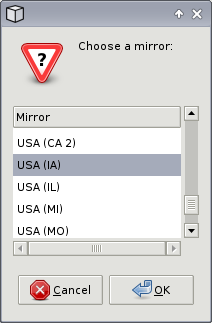
\includegraphics[width=2in]{cran-mirror.png}
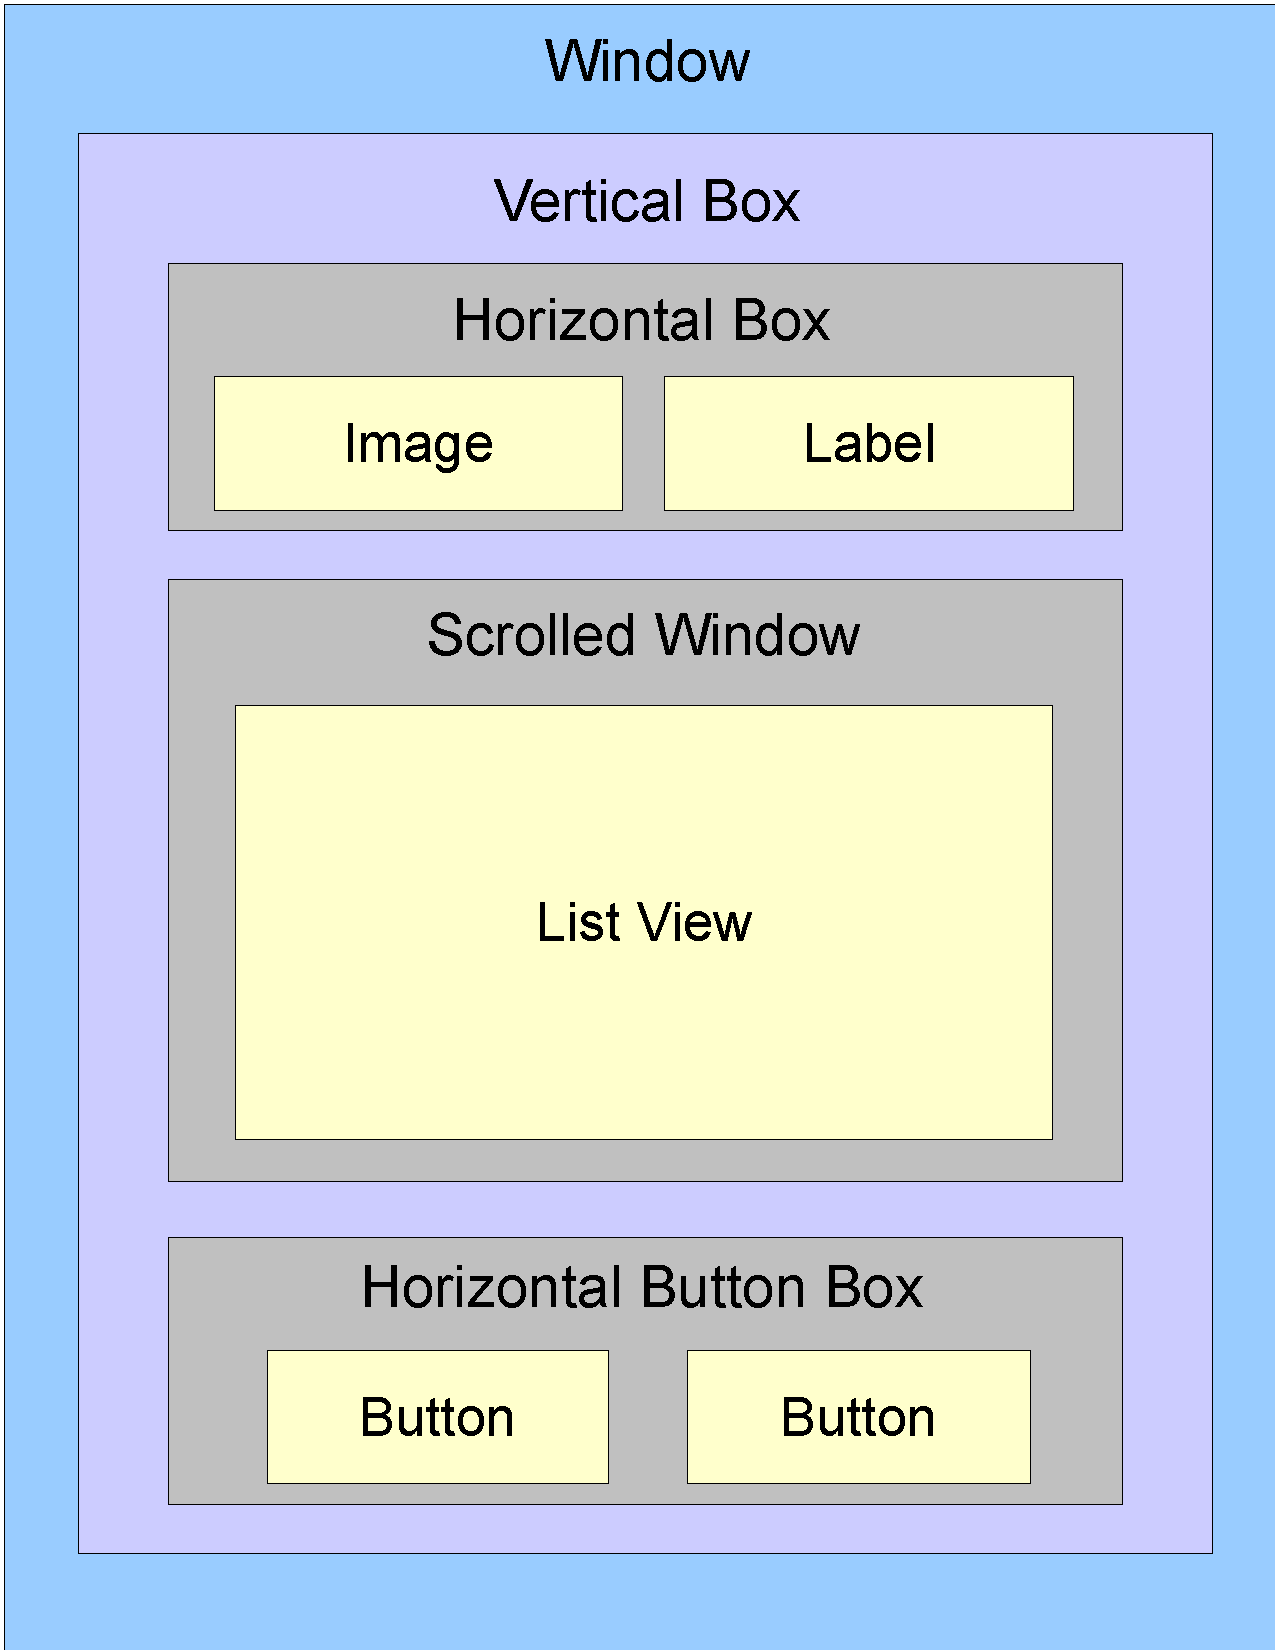
\includegraphics[width=2in]{widget-hierarchy.pdf}
\caption{\label{fig:cran-mirror}\label{fig:widget-hierarchy} 
A dialog for selecting a CRAN mirror constructed
using the RGtk2 package. The screenshot of the dialog is shown on the
left. The user selects a mirror from the list and clicks the
``OK'' button to confirm the choice.
Each rectangle in the diagram on the right corresponds to a widget in
the GUI. The window is at the top-level,
and each of the other widgets is geometrically contained within its
parent. Many of the container widgets are invisible in the
screenshot.}
\end{center}
\end{figure}

%DTL:  Strange that we refer first to figure 2 and then figure 1.
% Why not put figure 1 and 2 side-by-side in a single figure and label
% them a) and b).
% Also, the part of the widget hierarchy in Figure 1 doesn't really
% relate to the GUI in figure 2.
%ML: I placed the CRAN mirror GUI and the widget hierarchy together.
% They now come before the class hierarchy.
Figure \ref{fig:cran-mirror} shows a \pkg{GTK+} GUI that allows the
user to
select a CRAN mirror for downloading \proglang{R} packages.
This GUI is likely familiar to many \proglang{R} users, since a
similar interface
is present in the official Windows and Mac OS X \proglang{R} GUIs,
among others.
There are several different types of widgets in the CRAN mirrors GUI.
A
text label instructs the user to choose a mirror.  A list contains the 
names of the mirrors, and there are buttons for confirming or
canceling the choice. 
The interface is enclosed by another type of widget, a window. 

All of these widget types have functionality in common. For example,
they are
all drawn on the screen in a consistent style. To formalize this
relationship 
and to simplify implementation by sharing code
between widgets, \pkg{GTK+} defines an inheritance hierarchy for its
widget
types, or classes. A small portion of the \pkg{GTK+} class hierarchy
is shown
in Figure \ref{fig:class-hierarchy}. For specifying the hierarchy,
\pkg{GTK+} 
relies on \pkg{GObject}, a \proglang{C} library that implements a
class-based, single-inheritance 
object-oriented system.  Each type of \pkg{GTK+} widget is a
\pkg{GObject} 
class that inherits from the base \emph{GtkWidget} class which
provides the general characteristics shared by all widget classes,
e.g. properties giving the location, color; methods for hiding,
showing and painting the widget. A \pkg{GObject} 
class encapsulates behaviors that all instances of the class share. 
Each class has a single parent from which it inherits 
the behaviors of its ancestors. A class can override any of its
inherited behaviors.
A more detailed and technical explanation of \pkg{GObject} is
available in 
Section \ref{sec:primer}. 

\begin{figure}
\begin{center}
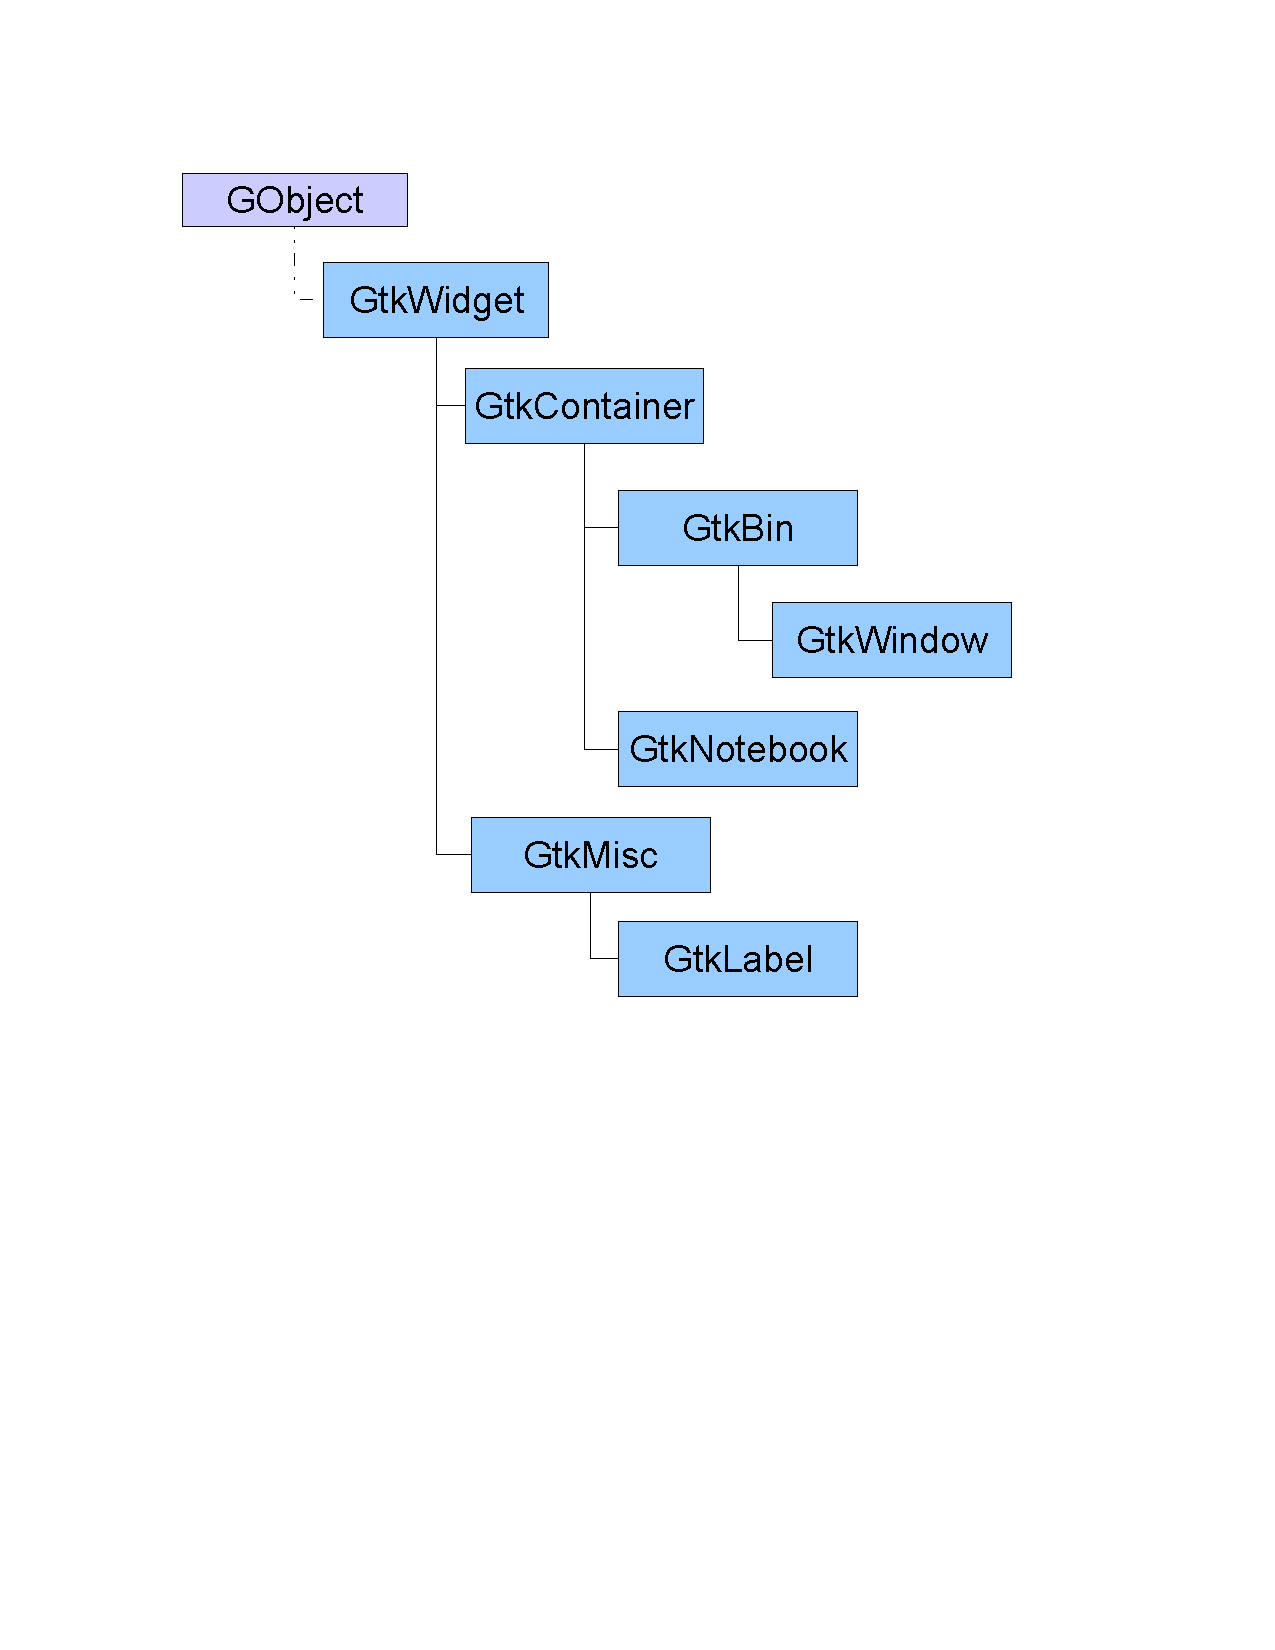
\includegraphics[width=3in]{class-hierarchy.pdf}
\caption{\label{fig:class-hierarchy}A small portion of the GTK+ class
hierarchy. 
All widgets are derived from the \emph{GtkWidget} class, which is
derived, 
indirectly, from the \emph{GObject} base class.}
\end{center}
\end{figure}

\subsubsection{The Widget Tree}

There is another tree hierarchy that is orthogonal to the 
class inheritance hierarchy. This hierarchy involves widget instances
rather
than widget classes. Each widget instance has a single parent
instance, except
for a top-level window which has none and serves as the root of the
tree. Child widgets are geometrically
contained by their parents. In Figure \ref{fig:cran-mirror}, 
for example, the label, list of mirrors, and buttons are all contained
within the 
top-level window, meaning that the window is the common ancestor of
the other widgets.
Figure \ref{fig:widget-hierarchy} shows, in a simplified way, the two
dimensional
nesting of the widgets in the mirror selection example. Widgets that
can contain 
other widgets are called \emph{containers} and their classes are
derived from 
the \emph{GtkContainer} class. Windows and tabbed notebooks are
examples of containers.
Combining primitive widgets like labels and icons within containers
leads to more complex displays, such as menus, toolbars and even
buttons which contain labels to display the text. A container is 
responsible for allocating its space to its children. This process is
called
layout management and is described in Section \ref{sec:layout}.



\subsection[GTK+ Widgets in R]{\pkg{GTK+} Widgets in \proglang{R}}

\pkg{RGtk2} provides an Application Programming Interface (API) to the
\pkg{GTK+} 
library. An API is a type of user interface where the user
is a programmer creating an application based on functions implemented
within a separate module. It is a contract that specifies in detail
the functionality available to a programmer without specifying how
that functionality is implemented. 
%DTL: I am not certain that continuing the Unwin & Hoffman definition
%of an interface helps as much here as saying that an API is like a
%contract that specifies in detail what is available to a programmer 
% but not how things are implemented.  It is a declaration rather than
% an interface.  I don't think identifying the module as a machine
% helps.
 
% ML: I added a sentence along the lines of it defining a contract. I
% would still argue, however, that an API is a user interface.

As with other user interfaces,
an API should be consistent and efficient to use. As an \proglang{R}
package,
\pkg{RGtk2} primarily aims to be consistent with \proglang{R}
conventions. This
means hiding aspects of the \pkg{GTK+} API that are foreign to
\proglang{R},
such as explicit memory management. A secondary concern is consistency 
with the underlying \pkg{GTK+} API. The developers of
\pkg{GTK+} have invested a significant amount of thought into its
design. Thus,
\pkg{RGtk2} endeavors to interface \proglang{R} to the virtual
entirety of \pkg{GTK+},
without leaving any gaps that may be unanticipated by the user. 
The only omissions are those that would violate consistency with
\proglang{R}. For example, functions related to explicit memory
management were excluded, as memory in \proglang{R} is managed by a
garbage collector. Array length parameters are also excluded, as the
length of a vector is always known in \proglang{R}.
%DTL: e.g.  some examples
The \pkg{RGtk2} API has also been designed for ease/efficiency of use.
Towards this end,
it specifies
a default value for a function parameter whenever sensible and uses a
special object-oriented syntax, as introduced by the SJava package
\citep{SJava}.
%DTL: RGtk didn't introduce the special syntax. It was first
%introduced in the SJava package.

To demonstrate the basic syntax and
features of the \pkg{RGtk2} API, we will construct a simple ``Hello
World'' GUI,
shown in Figure \ref{fig:hello-world}. 

\begin{figure}
\begin{center}
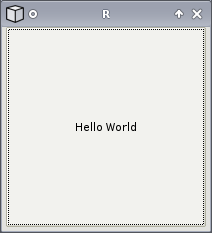
\includegraphics[width=2in]{hello-world.png}
\caption{\label{fig:hello-world}``Hello World'' in GTK+. 
A window containing a single button displaying a label with the text
``Hello World''.}
\end{center}
\end{figure}

We will gradually 
progress from this trivial GUI to the aforementioned CRAN mirrors GUI
and beyond.
The first step is to create a top-level window to contain our GUI.
Creating an instance of a \pkg{GTK+} widget requires calling a single
\proglang{R} 
function with its name matching the name of the class with the first
character in 
lowercase. The following statement constructs an instance of the
\emph{GtkWindow} class.
\begin{verbatim}
window <- gtkWindow("toplevel", show = FALSE)
\end{verbatim}

The first argument to the constructor for \emph{GtkWindow} corresponds
to the type of the window. The set of possible window types is
specified by what in \proglang{C} is known as an
\emph{enumeration}. Since enumerations are foreign to R, \pkg{RGtk2}
accepts string representations of enumeration values, like
``toplevel''. For every \pkg{GTK+} enumeration, \pkg{RGtk2} provides
an \proglang{R} vector that maps the nicknames to the underlying
numeric values.  In the above case, the vector is named
\emph{GtkWindowType}. It is rarely necessary to explicitly use the
enumeration vectors; specifying the nickname will work in most cases,
including all method invocations and is preferable as it is easier for
human readers to comprehend.

The \emph{show} argument is the last argument for every widget
constructor. It
indicates whether the widget should be made visible immediately after
construction.
The default value of \emph{show} is \emph{TRUE}. In this case we want
to
defer showing the window until after we finish constructing our simple
GUI.

%DTL: This next paragraph hangs out a little, i.e. it doesn't flow
%directly from the previous paragraphs but introduces a new concept
%and then we move on to another.  It is okay, but it would be nice to
%try to connect it a little more.
The next steps are to create a ``Hello World'' button and to place the
button in the window that we have already created. This depends on an
understanding of how of one programmatically interacts with widgets.
Each widget class defines an API 
consisting of methods, properties, fields and signals. Methods are
functions 
that take an instance of their class as the first argument and are
used to instruct the 
widget to perform an action. Properties and fields store the public
state of a widget. Examples of properties include the title of a
window, the label on a button, and whether a widget has the keyboard
focus. 
%DTL: e.g., give some examples.
Signals are emitted as a result of events, such as user interaction
with a widget.
%DTL: signals can be omitted by programmatic actions also.
By attaching an \proglang{R} handler function to a widget's signal, we
can
perform an action in response to all user inputs that generate that
signal. We explain how one can interface \proglang{R} functions with
each of these in the following sections as we continue with our
``Hello World'' example.

\subsubsection{Invoking Methods}

Methods are functions that operate on widgets inheriting from a
particular class.
The \pkg{RGtk2} function for each \pkg{GTK+} method is named according
to the 
\emph{classNameMethodName} pattern. For example, to add a child to a
container, we 
need to invoke the \emph{add} method on the \emph{GtkContainer} class. 
The corresponding function name would be \emph{gtkContainerAdd}.
However, this 
introduces an inefficiency in that the user needs to remember the
class to which
a method belongs. To circumvent this problem, we introduce a syntax
that is similar
to that found in various object-oriented languages. The widget
variable is given first, followed by the \$ operator, then the method
name and its arguments. This syntax for calling \emph{gtkContainerAdd}
is demonstrated 
below as we add a button with the label ``Hello World'' to our window.
The
third statement calls \emph{gtkWindowSetDefaultSize} to specify our
desired
size for the window when it is first shown. Each method belongs to a
separate
class, but the syntax frees the user from the need to remember the
exact classes
and also saves some typing.
\begin{verbatim}
button <- gtkButton("Hello World")
window$add(button)
window$setDefaultSize(200,200)
\end{verbatim}
Note that we use the lower case form of the first letter when using
the \$ syntax, but the upper case form in the
\emph{classNameMethodName} function name. The \$ acts as a word
separator and we use lower case at the beginning of new words.



\subsubsection{Accessing Properties and Fields}

Properties are self-describing elements that store the state of a
widget.
Examples of properties include the title of a window, whether a
checkbox is checked, and
the length in characters of a text entry box. The \proglang{R} subset
function 
\emph{[} may be used to get the value of a widget property by name.
Below we access the value of the \emph{visible} property of our
window. We
find that the value is \emph{FALSE}, since we specified it not to be
shown
at construction and have not made it visible since then.
\begin{verbatim}
> window["visible"]
[1] FALSE
\end{verbatim}

\pkg{Gtk+} properties may be set, given that they are writable, using
the regular R assignment operator (\emph{<-} or \emph{=}). This is
actually implemented via the \emph{[<-} method for \pkg{Gtk+} widgets
in \pkg{RGtk2}. The example below makes the window created above
visible, using the two property setting methods. In this particular
case, we could also show the window using the \emph{gtkWidgetShow}
method, which is more conventional.
\begin{verbatim}
window["visible"] <- TRUE # or
window$show()             # the conventional way
\end{verbatim}

For convenience, one might desire to set multiple properties with a
single statement.
This is possible using the \emph{gObjectSet} method, which behaves
similarly
to the \proglang{R} \emph{options} function, in that the argument name
indicates
the property to set to the argument value. 
%DTL: Perhaps make note that this is gObjectSet and not gtkObjectSet.
In the single statement below, we 
set the window icon to the RGtk logo image and set the title to
``Hello World 1.0''. 
The \emph{imagefile} function retrieves an image from the \pkg{RGtk2}
installation.
\emph{gdkPixbuf} returns a list, where the first element is a
\emph{GdkPixbuf}, an image object,
and the second is a description of an error encountered when reading
the file
or \emph{NULL} if the operation was successful. Here we assume that
there is no error.
\begin{verbatim}
image <- gdkPixbuf(filename=imagefile("rgtk-logo.gif"))[[1]]
window$set(icon = image, title = "Hello World 1.0")
\end{verbatim}

In rare cases, it is necessary to access a field in the widget data
structure.
Fields are different from properties in several ways. Most
importantly, it is
never possible to set the value of a field. The user can retrieve the
value of
a field using the \emph{[[} function. For example, now that our window
has been shown, it has been allocated a rectangle on the screen. This
is stored
in the \emph{allocation} field of \emph{GtkWidget}. It returns a list 
representing a \emph{GdkRectangle} with
elements \emph{x}, \emph{y}, \emph{width} and \emph{height}.
%DTL:  Why doesn't this have a class such as GdkRectangle. We are
%losing information about the object which is available from the
%property.

% ML: This appears to be a bug. It seems that some of the older 
% conversion routines that I implemented manually do not set the class
% attribute. Weird how I never noticed that.

\begin{verbatim}
> window[["allocation"]]
$x
[1] 0

$y
[1] 0

$width
[1] 200

$height
[1] 200
\end{verbatim}

\subsubsection{Handling Signals/Events}

Once a GUI is displayed on the screen, the user is 
generally free to interact with it. Examples of user actions include 
clicking on buttons, dragging a slider and typing text into an entry
box.
In the CRAN mirrors example, possible user actions include
selecting a mirror in the list, clicking the ``OK'' or ``Cancel''
buttons 
and pressing a keyboard shortcut, such as \texttt{Alt-O} for ``OK''. 
An application may wish to respond in a certain way to one or more of
such actions.
The CRAN mirrors application, for example, should respond to an ``OK''
response
by saving the chosen mirror in the session options.

So far, we have created and manipulated widgets by calling a list
of procedures in a fixed order. This is convenient as long as the
application
is ignoring the user. Listening to the user would
require a loop which continuously checks for user input.
It is not desirable to implement such a loop for every application, so
\pkg{GTK+} provides one for applications to use. When an application
initializes the \pkg{GTK+} event processing loop, there is an 
\emph{inversion of control}. The application no longer has primary
control
of its flow; instead, \pkg{GTK+} asynchronously informs the
application of 
events through the invocation of functions provided by the application
to 
handle a specific type of event. These handlers are known as 
\emph{callbacks}, because \pkg{GTK+} is calling back into the
application. 

\pkg{GTK+} widgets represent event types as signals. One or more
callbacks can be connected to a signal. When the event corresponding
to the
signal occurs, the signal is emitted and the callbacks are executed in
an order
depending on how they were connected. In order to execute \proglang{R}
code in 
response to a user action on a widget, we connect an \proglang{R}
function to the 
appropriate signal on the widget.  The \emph{gSignalConnect} function 
performs this connection. The following code will make our ``Hello
World'' 
example from above more interactive.
The call to \emph{gSignalConnect} will cause ``Hello World!'' to be
printed 
upon emission of the ``clicked'' signal from the button in our window.
The 
``clicked'' signal is emitted when the user clicks the button with a
pointer
device or activates the button with a keyboard shortcut.
\begin{verbatim}
gSignalConnect(button, "clicked", 
               function(widget) print("Hello world!"))
\end{verbatim}

\subsubsection{Documentation}

The \pkg{RGtk2} documentation is available using the conventional
\proglang{R} 
\emph{help} command. It is derived from the documentation of
\pkg{GTK+} itself.
To see the methods, properties, fields, and signals available
for a particular class, the user should access the help topic matching
the class name.
For example, to read the documentation on \emph{GtkWindow} we enter:
\begin{verbatim}
help(GtkWindow)
\end{verbatim}

Similarly, the detailed help for a specific method is stored under the
full
name of the function. For example, to learn about the \emph{add}
method on
\emph{GtkContainer}, we enter:
\begin{verbatim}
help(gtkContainerAdd)
\end{verbatim}

\subsection{Widget Layout}\label{sec:layout}

In our ``Hello World'' example, we added only a single widget, a
button, to the 
top-level window. In contrast, the CRAN mirrors window contains
multiple 
widgets, which introduces the problem of appropriately allocating the
space in a
window to each of its descendents. This problem is often called
\emph{layout management}.
Laying out a GUI requires specifying the position and size of each
widget below
the top-level window. The simplest type of layout management is
static; the
position and size of each widget are fixed to specific values. This is
possible
with \pkg{GTK+}, but it often yields undesirable results. A GUI is
interactive 
and changes in response to user input. The quality of a fixed layout
tends to decrease
with certain events, such as the user resizing
the window, a widget changing its size requirement, or the application
adding or removing widgets. For this reason, most layout management is
dynamic.

In \pkg{GTK+}, containers are responsible for the layout
of their children. Figure \ref{fig:widget-hierarchy} shows how the
nesting of 
layout containers results in the CRAN mirrors GUI shown in Figure 
\ref{fig:cran-mirror}. The example employs several important types of
\pkg{GTK+}
layout containers. First, there is the top-level \emph{GtkWindow} that
is derived from \emph{GtkBin}, which in turn derives from
\emph{GtkContainer}.
A \emph{GtkBin} holds only a single child, and \emph{GtkWindow} simply
fills all
of its allocated space with its child. The most commonly used
container
for holding multiple children is the general \emph{GtkBox} class,
which stacks its children
in a specified order and in a single direction, vertical or
horizontal. The 
children of a \emph{GtkBox} always fill the space allocated to the box
in the direction orthogonal to that of the stacking. The \emph{GtkBox}
class is abstract (or virtual), meaning that one cannot create
instances of it. Instead, we instantiate one of its non-abstract
subclassses.  For example, in the CRAN mirror GUI, a vertical box,
\emph{GtkVBox}, stacks the label above the list, and a horizontal
button box, \emph{GtkHButtonBox},
arranges the two buttons. \emph{GtkVBox} and its horizontal analog
\emph{GtkHBox}
are generic layout containers, while the button boxes
\emph{GtkVButtonBox} and 
\emph{GtkHButtonBox} offer facilities specific to the layout of sets
of buttons.
%DTL: perhaps mention that GtkBox is a virtual class of which we never
%create instances and we use the derived classes GtkHBox and GtkVBox.


Here we will explain and demonstrate the use of \emph{GtkHBox}, the
generic
horizontal box layout container. \emph{GtkVBox} can be used exactly
the same way;
only the direction of stacking is different. Figure \ref{fig:packing}
illustrates
a sampling of the possible layouts that are possible with a
\emph{GtkHBox}.

%DTL: It would be good to number the rows so that people can easily
%connect the descriptions in the text to the particular row.
\begin{figure}
\begin{center}
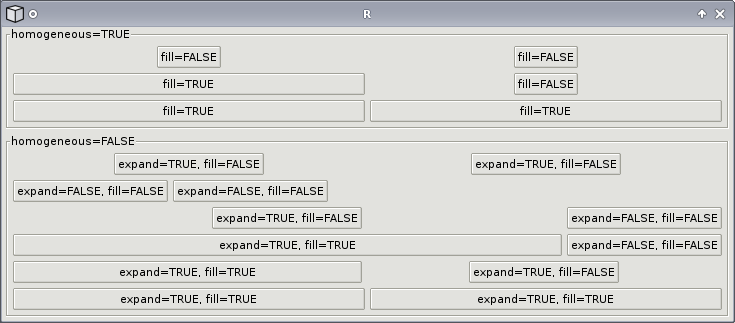
\includegraphics{packing.png}
\caption{\label{fig:packing}A screenshot demonstrating the effect of
packing two
buttons into \emph{GtkHBox} instances using the \emph{gtkBoxPackStart}
method 
with different combinations of the \emph{expand} and \emph{fill}
settings. 
The effect of the \emph{homogeneous} spacing setting on the
\emph{GtkHBox} is 
also shown.}
\end{center}
\end{figure}

The code for some of these layouts is presented here.
We begin by creating a \emph{GtkHBox} widget. We pass \emph{TRUE} for
the
first parameter, \emph{homogeneous}. This means every child will have
the
same amount of available space in the horizontal orientation. The
second 
parameter directs the box to leave 5 pixels of space between each
child. 
\begin{verbatim}
box <- gtkHBox(TRUE, 5)
\end{verbatim}
Making the space available to the children does not mean that the
children will fill it. That is specified by the \emph{fill} parameter
of the \emph{gtkBoxPackStart} and \emph{gtkBoxPackEnd} methods, which
pack a widget into a box with left and right justification (top and
bottom for a \emph{GtkVBox}), respectively. For this explanation, we
restrict ourselves to \emph{gtkBoxPackStart}, since
\emph{gtkBoxPackEnd} works the same except for the
%DTL: direction or justification?
justification. Below, we pack two buttons, \emph{button\_a} and
\emph{button\_b}, against the left side of the box. The space
distribution is homogeneous, but the extra space for each widget is
not filled. This results in the first row in Figure \ref{fig:packing}.
\begin{verbatim}
button_a <- gtkButton("Button A")
button_b <- gtkButton("Button B")
box$packStart(button_a, fill = FALSE)
box$packStart(button_b, fill = FALSE)
\end{verbatim}

In many cases, it is desirable to give children unequal amounts of
space.
This is evident in the CRAN mirrors dialog, where the mirror list is
given
priority over the ``Please choose a mirror:'' label in space
distribution.
To create an inhomogeneously spaced \emph{GtkHBox}, we pass
\emph{FALSE} as the first
argument to the constructor.
\begin{verbatim}
box <- gtkHBox(FALSE, 5)
\end{verbatim}
In an inhomongeneous layout, the widgets only take up their minimum
required
size, unless we pass \emph{TRUE} for the \emph{expand} parameter to
\emph{gtkBoxPackStart}. When a widget is packed to expand, its
available space
expands against the space given to the other children. Any space that
is
not consumed by the minimum size requirements of the children is
divided
equally among the expanding children. In the example below, the
\emph{button\_a}
expands against \emph{button\_b} and pushes \emph{button\_a} against
the right 
side of the box.
\begin{verbatim}
box$packStart(button_a, expand = TRUE, fill = FALSE)
box$packStart(button_b, expand = FALSE, fill = FALSE)
\end{verbatim}
The result is the sixth row from the top in Figure \ref{fig:packing}.
The
figure contains several other permutations of the \emph{homogeneous},
\emph{expand} 
and \emph{fill} settings.

\pkg{GTK+} contains many types of layout containers besides boxes,
including 
a grid layout (\emph{GtkTable}), a user-adjustable split pane
(\emph{GtkHPaned}
and \emph{GtkVPaned}), and a tabbed notebook (\emph{GtkNotebook}).
More types of
layout containers will be demonstrated later in the tutorial.

\section{Basic GUI Construction}

% a relatively simple first gui: dialogs (just a message, multiple
buttons)
% giving the user more choices: check button, radio buttons, combo box
in dialogs
% CRAN mirrors example (list dialog)
% alpha-slider (microarray) example
%   (approximiately) continuous choices: slider, (spin button)
%   displaying information as graphics: cairoDevice, mention
GtkDrawingArea
% spreadsheet app: 
%   advanced choosers: files, mention colors, fonts
%   displaying tabular information: tree view
%   arbitrary text input: text entry (completion)
%   advanced containers: 
%     space saving / hiding: menubar, toolbar, scrolled window,
notebook, (expander)
%     (letting the user decide: pane)
%   displaying status: statusbar (progressbar)
%   assisting the user: tooltips, (wizard)
% moving data around: dnd, clipboard

Thus far, we have reviewed the fundamentals of \pkg{GTK+}, working
with
\pkg{GTK+} widgets from \proglang{R}, and widget layout management. In
this
section, we will build on this foundation to create some basic but
potentially
useful GUIs. 

Constructing a GUI may be conceptually divided into two basic steps.
First, one must create the individual widgets, specify their
properties,
and organize them into containers. This defines the physical aspect
of the GUI: the appearance of the widgets and their spatial
organization.
The second step defines the behavior or the logical aspect of the
interface. It involves registering handlers for signals that are
emitted
by the widgets, for example in response to a user pressing a button.
The signal handlers encapsulate the logic beneath the interface. In
this
section, we will demonstrate these two steps and show how their
integration
results in functional GUIs.

\subsection{A Dialog with the User}\label{sec:dialog-example}

A user interface is the conduit for a conversation between the machine
and the
user. This conversation may be broken down into a series of exchanges
called 
\emph{dialogs}. An application often needs to make a specific request
for user input, such as the desired CRAN mirror. This type of dialog
is 
initiated by the machine sending a question to the user. The machine
then
waits for the user to respond. Usually, the application is unable to
continue
until receiving the user response, so the rest of the GUI is blocked
until
the dialog is concluded. This is called a \emph{modal} dialog.
A dialog is described as \emph{non-modal} when the user can continue
to perform other tasks even when the dialog is displayed.

\pkg{GTK+} explicitly supports modal and non-modal requests for user
input with a dialog widget, a top-level window that emits the
\emph{response} signal when the user has responded to the query. All
dialogs in \pkg{GTK+} are derived from the \emph{GtkDialog} class. The
CRAN mirrors GUI is an application of \emph{GtkDialog}. In the simpler
example below, we will create a dialog that asks whether the user
wants to upgrade the \pkg{RGtk2} package installed on the
system. Although we could build such a dialog using \emph{GtkDialog}
directly, \emph{GtkMessageDialog}, an extension of \emph{GtkDialog},
saves typing for queries that can be expressed with a textual message
and a set of buttons for the response. The dialog is constructed with
a single function call:
\begin{verbatim}
main_application_window <- NULL # for purposes of this example
dialog <- gtkMessageDialog(main_application_window,
"destroy-with-parent", 
  "question", "yes-no", "Do you want to upgrade RGtk2?")
\end{verbatim}
In the above invocation, the first parameter indicates the parent
window for
the dialog. It is assumed that the main window of the application is
stored 
as \emph{main\_application\_window}. The second parameter indicates
that
the dialog should be destroyed when its parent, the main window, is
destroyed.
The next parameter indicates that this is a ``question'' dialog, which
causes
the dialog to display a question mark icon to the left of the text.
The 
predefined set of buttons, in this case consisting of ``Yes'' and
``No'', 
is specified by the next parameter. The final parameter specifies the
message text.
The resulting dialog is shown in Figure \ref{fig:upgrade-dialog}.

\begin{figure}
\begin{center}
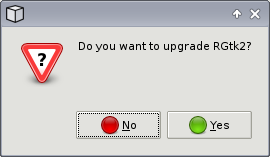
\includegraphics[width=3in]{upgrade-dialog.png}
\caption{\label{fig:upgrade-dialog}A screenshot of a message dialog
requesting a 
``Yes'' or ``No'' response from the user.}
\end{center}
\end{figure}

It is desirable for this dialog to be \emph{modal}, meaning that the
focus
is restricted to the dialog window until the user responds to the
question. By
invoking the \emph{gtkDialogRun} function, the dialog becomes modal
and execution
is blocked until the user gives a response, which is returned from the
function.
If the user answered ``Yes,'' the latest version of \pkg{RGtk2} will
be 
installed. The call to \emph{gtkWidgetDestroy} closes the dialog
window and 
renders it unusable.
\begin{verbatim}
if (dialog$run() == GtkResponseType["yes"])
 install.packages("RGtk2")
dialog$destroy()
\end{verbatim}
The reference to \emph{GtkResponseType} above is one of the rare cases
in which
it is necessary to access an enumeration vector to retrieve the
numeric value
for a nickname. The reason for this is that
\emph{gtkDialogGetResponse} returns
a plain numeric value to avoid an unnecessary restriction on the
number of 
possible response types from a dialog. In this case, it is known from
the documentation of \emph{GtkMessageDialog} that the value
corresponding to
the user clicking the ``Yes'' button will equal the ``yes'' value in
\emph{GtkResponseType}.

\subsection{Giving the User More Options}
% toggle button, radio buttons, combo box

Applications often need to ask questions for which a simple ``Yes'' or
``No'' answer does not suffice. As the number of possible responses to
a query increases, enumerating every response with a button would
place a burden on the user; it is easy to make a mistake when choosing
one response from many. An interface should be forgiving and allow the
user to confirm the choice before proceeding.  This is how the CRAN
mirrors dialog behaves: if the user accidentally chooses a mirror on
the other side of the world, the user can correct the choice before
clicking the ``Okay'' button and starting the installation
process. This relates to the common need for a program to issue a set
of queries to the user. Separating each query into its own dialog of
buttons may unnecessarily force the user to answer the questions in a
fixed, linear order and may not be very forgiving. It would also leave
the user without a sense of context. If there were many actions and
choices available to the user, a dialog-based interface would be
tedious to use, requiring the user to click through dialog after
dialog. Instead, a less assertive, non-linear interface is desired. In
the examples below, we demonstrate widgets that present options in a
passive way, meaning that there is usually no significant, immediate
consequence to user interaction with the widget and the user has to
conclude the interaction by clicking either the ``Okay'' or ``Cancel''
button.

The simplest user-level choice is binary and is usually represented in
a passive
way by a checkbox. In \pkg{GTK+}, the checkbox class is the
\emph{GtkCheckButton}. We may wish to extend our dialog confirming the
upgrade of \pkg{RGtk2} to include the option of also upgrading the
\pkg{GTK+} library. In the snippet below, we achieve this by adding a
check button to the dialog.  The area above the buttons in the
\emph{GtkDialog} is contained within a \emph{GtkVBox}, which is stored
as a field named \emph{vbox}. Figure \ref{fig:checkbox-dialog} shows
our custom checkbox dialog.
\begin{verbatim}
dialog <- gtkMessageDialog(main_application_window,
"destroy-with-parent", 
  "question", "yes-no", "Do you want to upgrade RGtk2?")
check <- gtkCheckButton("Upgrade GTK+ system library")
dialog[["vbox"]]$add(check)
\end{verbatim}

\begin{figure}
\begin{center}
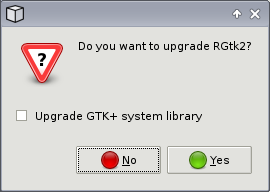
\includegraphics[width=3in]{checkbox-dialog.png}
\caption{\label{fig:checkbox-dialog}A screenshot of a message dialog
with a 
check box for requesting additional input on top of the
original dialog in Figure \ref{fig:upgrade-dialog}.}
\end{center}
\end{figure}

Let us now suppose that we would like to give the user the additional
option of
installing a development (experimental) version of \pkg{GTK+}.
When an option has several choices, a check button is no longer
adequate. A
simple extension is to create a set of toggle buttons where only one
button
may be active at once. The buttons in this set are known as
\emph{radio buttons}.
Below, we create a new dialog that asks the user to specify the
version of \pkg{GTK+}
to install, if any. When each radio button is created, it needs to be
given the existing buttons
in the group. For creating the first button, \emph{NULL} should be
passed as the group.
Each button is added to a vertical box. 
\begin{verbatim}
dialog <- gtkMessageDialog(main_application_window,
"destroy-with-parent", 
  "question", "yes-no", "Do you want to upgrade RGtk2?")
choices <- c("None", "Stable version", "Unstable version")
radio_buttons <- NULL
vbox <- gtkVBox(FALSE, 0)
for (choice in choices) {
  button <- gtkRadioButton(radio_buttons, choice)
  radio_buttons <- c(radio_buttons, button)
  vbox$add(button)
}
\end{verbatim}
A group of radio buttons are often graphically enclosed by a drawn
border with a text label indicating the purpose of the buttons. This
widget is a container 
called \emph{GtkFrame} and is generally used for graphically grouping
widgets that are
logically related. The code below adds the box containing the radio
buttons
to a frame.
%DTL: need to explain what a frame is and connect it to the frame
widget.
%ML: isn't this done above or do you mean more information?
The final result is shown in Figure \ref{fig:radio-dialog}.
\begin{verbatim}
frame <- gtkFrame("Install GTK+ system library")
frame$add(vbox)
dialog[["vbox"]]$add(frame)
\end{verbatim}

\begin{figure}
\begin{center}
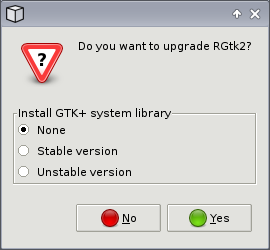
\includegraphics[width=3in]{radio-dialog.png}
\caption{\label{fig:radio-dialog}A screenshot of a message dialog with
a set of
radio buttons on top of the base dialog shown in Figure
\ref{fig:upgrade-dialog}.}
\end{center}
\end{figure}

Now we would like to go a step further and allow the user to choose
the exact series of \pkg{GTK+} to install, as \pkg{RGtk2} is source
compatible with any version after $2.8.0$. As the number of options
increases, however, radio buttons tend to consume too much space on
the screen. In
this case, a label displaying the current selection with a drop down
menu allowing for selecting from a list of alternatives may be
appropriate.  This is known as a \emph{GtkComboBox} in \pkg{GTK+}. The
following snippet illustrates its use. Each call to
\emph{gtkComboBoxAppendText} adds a text item to the drop-down
menu. The call to \emph{gtkComboBoxSetActive} makes the first item the
selected one. Figure \ref{fig:combo-dialog} shows the result.
\begin{verbatim}
dialog <- gtkMessageDialog(main_application_window,
"destroy-with-parent", 
  "question", "yes-no", "Do you want to upgrade RGtk2?")
choices <- c("None", "GTK+ 2.8.x", "GTK+ 2.10.x", "GTK+ 2.12.x")
combo <- gtkComboBoxNewText()
combo$show()
for (choice in choices) 
  combo$appendText(choice)

combo$setActive(0) # select "None", the first choice.
frame <- gtkFrame("Install GTK+ system library")
frame$add(combo)
dialog[["vbox"]]$add(frame)
\end{verbatim}

\begin{figure}
\begin{center}
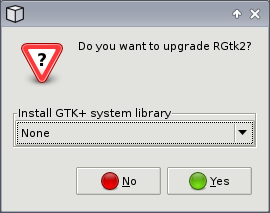
\includegraphics[width=3in]{combo-dialog.png}
\caption{\label{fig:combo-dialog}A screenshot of a message dialog with
a 
combobox for selecting an option from a drop-down menu before
responding to
the dialog.}
\end{center}
\end{figure}

\subsection{The CRAN Mirrors Dialog}

Having demonstrated the creation some basic dialogs, we are now
prepared to 
construct the CRAN mirror selection dialog, shown
in Figure \ref{fig:cran-mirror}.
Given the large number of CRAN mirrors, one strategy would be to 
borrow the combobox dialog created above; however, there may be a
better 
alternative. Since their is no reasonable default CRAN mirror, the
user always
needs to pick a mirror. Packing the mirrors into a combo box would
only force 
the user to make an extra click. Instead, we want to display a
reasonable
number of CRAN mirrors immediately after the dialog is opened. It may
not be possible to display every mirror at once on the screen, but, as
seen
in the screenshot, we can embed the list in a scrolled box, so that
only
one part of the list is visible at a given time.

We begin with the construction of the dialog window. For this dialog,
we 
assume that there is no main application window (see Section
\ref{sec:spreadsheet-example}) to serve as the
parent. 
%DTL: The concept of an application window needs more explanation.
% It is defined in section 4 (Sample Application).
Instead, we pass \emph{NULL} for the parent and $0$ for the second
argument 
rather than \emph{``destroy-with-parent''}.
\begin{verbatim}
dialog <- gtkMessageDialog(NULL, 0, "question", "ok-cancel", 
                            "Choose a mirror:", show = FALSE)
\end{verbatim}
Next, we create a list for holding the mirror names using the
\emph{GtkTreeView}
widget (so named because the rows in the list may be organized hierarchically, but we will not discuss this feature).  \pkg{RGtk2}
provides a 
facility for creating a flat tabular data structure based on an
\proglang{R}
\emph{data.frame}, called \emph{RGtkDataFrame}. \emph{RGtkDataFrame}
is
an extension of \emph{GtkTreeModel}, which is the data structure
viewed by
\emph{GtkTreeView}. Below, we create an \emph{RGtkDataFrame} for our
list
of CRAN mirrors and construct a \emph{GtkTreeView} based on it.
\begin{verbatim}
mirrors <- read.csv(file.path(R.home("doc"), "CRAN_mirrors.csv"),
as.is = TRUE)
model <- rGtkDataFrame(mirrors)
view <- gtkTreeView(model)
\end{verbatim}
%DTL: This next bit is very detailed and specific relative to all the
%text in the document up until this point.
%ML: I included this explanation, because the GtkTreeView is very 
%complex. To really understand what is going on, even when just
%creating a simple list, one needs a complete explanation.
Initially, the tree view does not contain any columns. We need to
create a \emph{GtkTreeViewColumn} to list the mirror names. A
\emph{GtkTreeViewColumn}
is a \emph{GtkCellLayout}, which is a container of
\emph{GtkCellRenderer}s. 
A \emph{GtkCellRenderer} is not a widget; it is responsible for
rendering
a portion of every cell in a column. Its rendering is defined by a set
of
properties, each of which may be linked to a column in the data model
being displayed. For each
cell in a column, the cell renderer determines each of its data-linked
visual
properties from the value in the data model at the current
row and the column associated with the property. For simply displaying
text in a table, we use a \emph{GtkCellRendererText} and link its
\emph{text}
property to the column in the data containing the text we want to
display.
In this case, we want to display the first column of the
\emph{data.frame},
which is column $0$ to the \emph{GtkTreeView}.
\begin{verbatim}
column <- gtkTreeViewColumn("Mirror", gtkCellRendererText(), text = 0)
view$appendColumn(column)
\end{verbatim}
Given the large number of CRAN mirrors, the list would take up
excessive space
if not embedded into a scrolled window. \emph{GtkScrolledWindow} is a
container 
widget that provides a scrolled view of its child when the child
requests more
space than is available. We add the tree view to a
\emph{GtkScrolledWindow} 
instance that requests a minimum vertical size sufficient for showing
several 
mirrors at once.
\begin{verbatim}
scrolled_window <- gtkScrolledWindow()
scrolled_window$setSizeRequest(-1, 150)
scrolled_window$add(view)
\end{verbatim}
It only remains to add the scrolled window to the dialog, run the
dialog, and
set the selected CRAN mirror if the user confirms the selection. The
selection
of a tree view is stored in a separate \emph{GtkTreeSelection} object
retrieved
by \emph{gtkTreeViewGetSelection}. The \emph{getSelectedRows} method
returns a 
list containing the tree paths for the selected rows and the tree
model. The 
list of tree paths is stored under the name \emph{retval} as it is the
actual
return value from the \proglang{C} function. Finally, we retrieve the
row index
from the \emph{GtkTreePath} for the first (and only) selected row and
set its 
URL as the repository.
\begin{verbatim}
dialog[["vbox"]]$add(scrolled_window)
if (dialog$run() == GtkResponseType["ok"]) {
  selection <- view$getSelection()
  sel_paths <- selection$getSelectedRows()$retval
  sel_row <- sel_paths[[1]]$getIndices()[[1]]
  options(repos = mirrors[sel_row, "URL"])
}
dialog$destroy()
\end{verbatim}

\subsection{Embedded R Graphics}\label{sec:embedded-graphics}

In a statistical graphical interface, it is often beneficial or
necessary to display statistical graphics within the interface. As
an example, we consider the contemporary problem of visualizing
micoarray data. The large number of genes leads to a significant
amount of overplotting when, for example, plotting the expression
levels from two chips in a scatterplot. One solution to the problem of
overplotting is alpha blending. However, choosing the ideal alpha
level may be time-consuming and tedious. Linking a slider widget to
the alpha level of an \proglang{R} scatterplot may accelerate the
search (See Figures \ref{fig:rgtk2-demo-initial} and
\ref{fig:rgtk2-demo-final}).


%DTL:  The different color doesn't show up too well here, which is of
course the point. But we should either say this or use a different
value (e.g. .5) or use color.

%ML: I am not sure what you mean by this.

\begin{figure}
\begin{center}
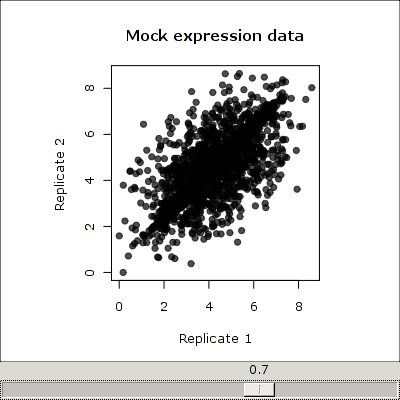
\includegraphics[width=3in]{demo-alpha-random-07-3}
\caption{\label{fig:rgtk2-demo-initial}Scatterplot of two microarray
replicates,
with a slider widget underneath that controls the alpha level of the
points. This screenshot shows the initial alpha of $0.7$.}
\end{center}
\end{figure}

\begin{figure}
\begin{center}
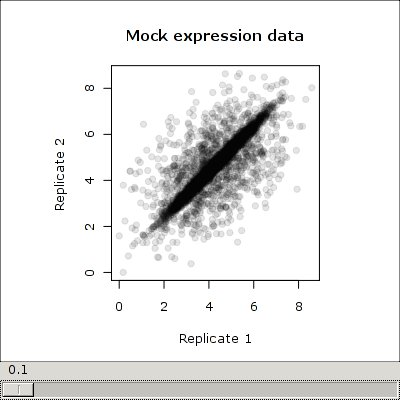
\includegraphics[width=3in]{demo-alpha-random-01-3}
\caption{\label{fig:rgtk2-demo-final}The same scatterplot from 
\ref{fig:rgtk2-demo-initial}, except the alpha has been set to to
$0.1$.}
\end{center}
\end{figure}

As a preliminary step, we use a 2D mixture distribution of correlated
variables
to emulate expression values for two microarray chips. 
\begin{verbatim}
n <- 5000
backbone <- rnorm(n)
ma_data <- cbind(backbone+c(rnorm(3*(n/4),sd=0.1), rt(n/4, 80)), 
  backbone+c(rnorm(3*(n/4),,0.1), rt(n/4, 80)))
ma_data <- apply(ma_data, 2, function(col) col - min(col))
\end{verbatim}

The first step towards making our GUI is to create the window that
will contain everything. 
\begin{verbatim}
win <- gtkWindow(show = FALSE)
\end{verbatim}

One may embed \proglang{R} graphics within an \pkg{RGtk2} GUI using
the 
\pkg{cairoDevice} \citep{cairoDevice} or \pkg{gtkDevice}
\citep{gtkDevice}
packages. The \pkg{cairoDevice} package draws \proglang{R} graphics
using 
\pkg{Cairo} \citep{cairo}, a library for vector-based, antialiased
graphics.
When \pkg{cairoDevice} draws to the screen it is actually drawing to a 
\pkg{GTK+} widget called \emph{GtkDrawingArea}. A
\emph{GtkDrawingArea}
is an empty widget meant for drawing arbitrary graphics in an
interface. Here we 
construct a drawing area in which the \proglang{R} graphics will be
drawn:
\begin{verbatim}
graphics <- gtkDrawingArea()
\end{verbatim}

Now that we have a widget for displaying \proglang{R} graphics, we
need the slider that controls the alpha level. A slider is a widget,
much like a scroll bar, for choosing a number at a certain precision
from a certain range. Here, a horizontal slider, called
\emph{GtkHScale}, is created with to range from 0.1 to 1.0, with a
step size of 0.1.
\begin{verbatim}
slider <- gtkHScale(min=0.1, max=1.00, step=0.1)
\end{verbatim}

When the user moves the slider, the plot should be updated so that its
alpha
level reflects the slider value. This is achieved by connecting
an \proglang{R} callback function to the ``value-changed'' signal of
the slider. 
This callback function, \emph{scale\_cb}, replots the microarray data,
\emph{ma\_data}, using
an alpha level equal to the current value of the slider. 
\begin{verbatim}
scale_cb <- function(range) 
              plot(ma_data[,1], ma_data[,2], 
                   col = rgb(0, 0, 0, alpha = range$getValue()),
                   xlab = "Replicate 1", ylab = "Replicate 2", 
                   main = "Mock expression data", pch = 19)
gSignalConnect(slider, "value-changed", scale_cb)
\end{verbatim}
%DTL: It would be good to address the issues of global variables and
%the use of closures.
%ML: It seems you have well-formed thoughts on that issue; could you
please add something?

The next steps are to add the drawing area and the slider to the
window and then to show the window on the screen. Although the window
is a
container, it inherits from \emph{GtkBin}, meaning that it can hold
only
a single child widget. Thus, we will pack our widgets into a vertical
stacking 
box container, \emph{GtkVBox}, and add our box to the window.
Here, we would like the graphics to take up all of the space not
consumed by the
slider, so the graphics device is packed to \emph{expand} and
\emph{fill}, while
the slider is not.
\begin{verbatim}
vbox <- gtkVBox()
vbox$packStart(graphics, expand = TRUE, fill = TRUE, padding = 0)
vbox$packStart(slider, expand = FALSE, fill = FALSE, padding = 0)
win$add(vbox)
\end{verbatim}

As a final step, we set the default size of the window and show it and
all of its children.
\begin{verbatim}
win$setDefaultSize(400,400)
win$showAll() 
\end{verbatim}

Now that the window is visible on screen, we can instruct \proglang{R}
to draw
its graphics to the drawing area. Using the \emph{asCairoDevice}
function, it is possible
to tell \pkg{cairoDevice} to draw to our \emph{GtkDrawingArea} widget
created above.
\begin{verbatim}
require(cairoDevice)
asCairoDevice(graphics)
par(pty = "s")
\end{verbatim}
The call to \emph{asCairoDevice} makes an R graphics device from this
widget and makes this the currently active graphics device on which R
graphics will be displayed.

Finally, the value of the slider is initialized to $0.7$,
\begin{verbatim}
slider$setValue(0.7)
\end{verbatim}
which in turn activates the callback, generating the initial plot. The
initial state of the interface is shown in Figure
\ref{fig:rgtk2-demo-initial}.  Figure \ref{fig:rgtk2-demo-final} shows
the plot after the user has moved the slider to set the value of alpha
to $0.1$.


\section{A Sample Application}\label{sec:spreadsheet-example}

The interfaces presented thus far are each designed for a singular,
focused task, such as choosing a CRAN mirror or viewing a scatterplot
at different alpha levels.  However, often an interface supports a
larger scope of different operations and the user is in control of
initiating different tasks from the general interface. These
interfaces for broader, more complex
applications are typically based on what is called an
%DTL: Here we define application window, yet we referred to it
earlier.
\emph{application window}, which often contains a menubar, toolbar,
application-specific area, and statusbar in order from top to
bottom. The menubar and toolbar are widgets designed to facilitate the
user selecting different \emph{actions}, each of which represents an
option or operation in the application.  The statusbar at the bottom
commonly reports the status of the application or information for the
user as a text message and may be adjacent to a progressbar that
monitors the progress of long running operations.  This layout and
design is a common convention which helps users navigate a new GUI.


This example demonstrates how one might construct a reasonably complex
application using \pkg{RGtk2}. We aim to build a viewer for one or
more R \emph{data.frame}s that is capable of sorting and filtering the
rows in each data frame. We also give it facilities to load and save a
\emph{data.frame} to and from a CSV file. 

The resulting GUI is shown in Figure \ref{fig:spreadsheet}. The data
is displayed in a table, using a \emph{GtkTreeView} widget. As we would like to support multiple spreadsheets at once, we embed each table in a tabbed notebook, \emph{GtkNotebook}. Below each spreadsheet is a text entry, \emph{GtkEntry}, in which the user may enter an expression for filtering the table view. Below this is a statusbar,
\emph{GtkStatusbar}, that communicates the status of the application
to the user, such as whether the loading of a dataset is complete. At
the top are a menubar (\emph{GtkMenubar}) and toolbar
(\emph{GtkToolbar}) that allow the user to invoke various actions,
such as loading a new dataset or quitting the application.

%DTL: the reader has to pull together the different parts in the next
%few pages.  It would be very valuable to provide a brief high-level
overview of
%the steps involved and how they piece together and then go into the
%details.

% ML: I hope the paragraph above rectifies this.

% As it stands, this looks quite involved and will be intimidating.
% As for the XML, I think mentioning that is a big mistake.

% ML:
% I was intending for this example to be complex, in order to satisfy
% the readers that want to write a similar application in R. I thought
% the previous examples were sufficient to help users get started.
% Granted, there is a jump here, but I'm trying to satisfy a broad
% spectrum of readers.

\begin{figure}
\begin{center}
%DTL:  The number of decimal places in this figure is way too
%much. Only wt has some values with 3 digits after the decimal.  So
% the remaining 3 are spurious, suggesting greater precision than the
% data support and for all the other variables, there are 4 or more
% unnecessary digits which serve only to obscure the meaningful ones.
%ML: This is a difficult problem to solve. Either we convert the data
% to a string ourselves (which would break eg sorting) or add an R
% handler to do the conversion on the fly (more complicated and slow).
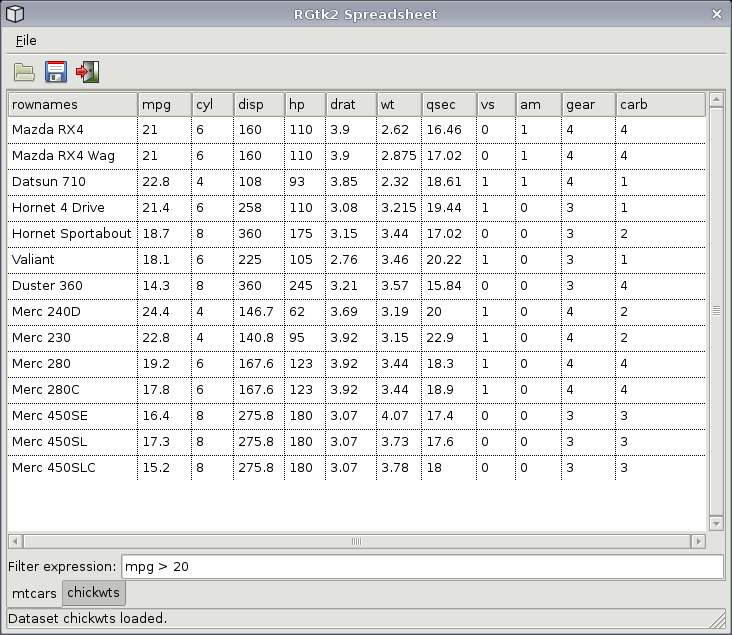
\includegraphics[width=6in]{spreadsheet.png}
\caption{\label{fig:spreadsheet}Screenshot of a spreadsheet
application 
constructed with RGtk2. The current sheet is from the \emph{mtcars}
dataset. The
table is filtered by the expression \texttt{mpg > 20} and sorted by
\emph{mpg}
in decreasing order.}
\end{center}
\end{figure}

We begin by creating the main window for the application and setting
its default size.
\begin{verbatim}
main_window <- gtkWindow(show = FALSE)
main_window["title"] <- "RGtk2 Spreadsheet"
main_window$setDefaultSize(600,600)
\end{verbatim}

Next, we implement the operations for the menu actions to load and
save a data frame and to quit the ``application''. Each of these
functions is a callback which takes the widget associated with the
action as its first argument and the top-level window as its
second. The load and save operations leverage the
\emph{GtkFileChooserDialog} widget type, a dialog that contains a
graphical file browser for specifying the path to a
file. \emph{GtkFileChooserDialog} has several modes corresponding to
common file selection tasks. In this case, we use the ``open'' mode
for the open action and the ``save'' mode for the save action. The
``accept'' response from the dialog indicates that the user has
confirmed the file selection by clicking the ``Open'' or ``Save''
button.
\begin{verbatim}
open_cb <- function(widget, window)  
{
  dialog <- gtkFileChooserDialog("Choose a CSV file", window, "open",
                                 "gtk-cancel",
GtkResponseType["cancel"],
	      	                 "gtk-open",
GtkResponseType["accept"])
  if (dialog$run() == GtkResponseType["accept"]) {
    df <- read.csv(dialog$getFilename())
    load_spreadsheet(df, basename(dialog$getFilename()))
  }
  dialog$destroy()
}
save_cb <- function(widget, window) {
  dialog <- gtkFileChooserDialog("Enter a name for the file", window,
"save",
                                 "gtk-cancel",
GtkResponseType["cancel"],
          	                 "gtk-save",
GtkResponseType["accept"])
  if (dialog$run() == GtkResponseType["accept"])
    save_file(dialog$getFilename()) # not implemented
  dialog$destroy()
}
quit_cb <- function(widget, window) 
              window$destroy() # quick and dirty

\end{verbatim}

We make these action callbacks accessible available in both the
menubar and toolbar. We begin by creating the main window, defining
the actions and bundling them into a \emph{GtkActionGroup}.  A
\emph{GtkActionGroup} is a container for \emph{GtkAction} objects. 
%DTL: I think the concept of a GtkAction needs more description here,
% just the basic idea.
The base \emph{GtkAction} represents an operation that a user may
request an application to perform. An action may be manifested in a
GUI in multiple ways, such as an item in a menu or a button in a
toolbar. The widgets are synchronized with the properties of the
action. For example, if an action is disabled, the menu items and
toolbar buttons will also be disabled. Extensions of \emph{GtkAction}
exist for toggle and radio options, but those are not described here.
\begin{verbatim}
actions <- list(
  list("FileMenu", NULL, "_File"), 
  list("Open", "gtk-open", "_Open File", "<control>O", 
       "Select a CSV file to load as a spreadsheet", open_cb),
  list("Save", "gtk-save", "_Save", "<control>S", 
       "Save the current spreadsheet to a CSV file", save_cb),
  list("Quit", "gtk-quit", "_Quit", "<control>Q", "Quit the
application", quit_cb)
)
action_group <- gtkActionGroup("spreadsheetActions")
action_group$addActions(actions, main_window)
\end{verbatim}
Each action is defined with a list, containing the action ID,
% Is this for referring to it later or the label that appears in the
% toolbar and/or menubar?
stock icon ID,
label, keyboard shortcut, tooltip, and callback.
%DTL:  If the FileMenu element is a container for the Open, Save and
% Quit elements, why aren't they elements of the FileMenu list.
% This flat structure to represent a hierarchy seems odd.
%ML: In GTK+, the actions are not organized hierarchically - that is
% specified in the layout (which is parsed from XML).
This is an example of 
high-level type conversion, where a native \proglang{R} structure is
implicitly converted to a complex \pkg{GTK+} object. In this case, an
\proglang{R} list is being converted to a set of \emph{GtkAction}
objects. See Section \ref{sec:high-level-conversion} for
a technical explanation and justification. The first action will serve
as the menu shell
%DTL: this is vague and undefined so please explain.
for the rest of the actions. Since it performs no
function, it is not necessary to specify all of the fields. 

We then create a \emph{GtkUIManager} and provide it with our action group.
\begin{verbatim}
ui_manager <- gtkUIManager()
ui_manager$insertActionGroup(action_group, 0)
\end{verbatim}
Next, we specify
the layout of the menubar and toolbar containing the actions defined
above, by calling the \emph{gtkUIManagerAddUi} method. Each piece of
UI added to a \emph{GtkUIManager} instance must be identified by a
``merge id''. This allows removing (unmerging) the UI at a later time.
The \emph{path} parameter indicates where the UI element should be
merged. Similar to a path in a URL, each element name in the path is
delimited by a forward slash (``/''). The \emph{name} parameter
identifies the element to the manager, and \emph{action} is the ID of
the action in the provided action group. If \emph{action} is NULL, a
separator widget is added. Finally, \emph{type} indicates the type of
UI element, such as a toolbar or menubar. The default is ``auto'',
which asks the \emph{GtkUIManager} to guess based on the path.
%DTL:  Boy, this seems very odd. Why an R programmer would switch to
%XML to express something that is easily specified in R is bizarre.
% I think you will really turn people off with this. Some people have 
% a strong  (often unfounded) objection to XML and this will allow
% them to discard RGtk2.  The XML is a red-herring. And it makes for
% a very big discontinuity in the programming style for creating a
% GUI, changing syntax, etc.
%ML: I've changed this to use the low-level API
% It's not as pretty but will keep everything in R.
% Could try to express a subset of it as a list... not sure.
\begin{verbatim}
merge <- ui_manager$newMergeId()
ui_manager$addUi(merge_id = merge, path = "/", name = "menubar",
                 action = NULL, "menubar")
ui_manager$addUi(merge, "/menubar", "file", "FileMenu", "menu")
ui_manager$addUi(merge, "/menubar/file", "open", "Open", "menuitem")
ui_manager$addUi(merge, "/menubar/file", "save", "Save", "menuitem")
ui_manager$addUi(merge, "/menubar/file", "sep", NULL, "menuitem")
ui_manager$addUi(merge, "/menubar/file", "quit", "Quit", "menuitem")
ui_manager$addUi(merge, "/", "toolbar", NULL, "toolbar")
ui_manager$addUi(merge, "/toolbar", "open", "Open", "toolitem")
ui_manager$addUi(merge, "/toolbar", "save", "Save", "toolitem")
ui_manager$addUi(merge, "/toolbar", "quit", "Quit", "toolitem")
\end{verbatim}
It is also possible to specify the layout of the actions using an XML
description. This may be desirable in more complex applications, where
the benefit of the declarative nature of XML outweighs the complexity
of mixing languages.

The next step is to use the \emph{GtkUIManager} to create the actual menubar and toolbar widgets from the action definitions and layout.
\begin{verbatim}
menubar <- ui_manager$getWidget("/Menubar")
toolbar <- ui_manager$getWidget("/Toolbar")
# so keyboard shortcuts work
main_window$addAccelGroup(ui_manager$getAccelGroup()) 
\end{verbatim}

To report the status of the application, we will use a
\emph{GtkStatusbar}. 
A statusbar maintains a stack of text messages and displays the
message
on top of the stack. Each message is associated with a \emph{context}.
A context
ID may be created using the \emph{gtkStatusbarGetContextId} function.
Here we create a 
statusbar and push the message ``Ready'' onto the top of the stack
within
the ``info'' context. Other contexts could be ``warning'' or
``error''; a context
can be created for any string.
\begin{verbatim}
statusbar <- gtkStatusbar()
info <- statusbar$getContextId("info")
statusbar$push(info, "Ready") 
\end{verbatim}
In order to handle multiple spreadsheets simultaneously but display
only one at a time, we will use a special type of container called
\emph{GtkNotebook}.  This provides labels on the border of the
notebook like a ring binder which the user can select to switch
between the different widgets within the notebook.  This is used in
Excel to present several work sheets within a single window, and also
within certain Web browsers to allow the user to view multiple Web
pages within a single window. Below, we create the notebook and add
it, along with the menubar, toolbar and statusbar, to the window,
through a \emph{GtkVBox}.
\begin{verbatim}
notebook <- gtkNotebook()
notebook$setTabPos("bottom") # tabs horizontally along the bottom
vbox <- gtkVBox(FALSE, 0)
vbox$packStart(menubar, FALSE, FALSE, 0)
vbox$packStart(toolbar, FALSE, FALSE, 0)
vbox$packStart(notebook, TRUE, TRUE, 0)
vbox$packStart(statusbar, FALSE, FALSE, 0)
main_window$add(vbox)
main_window$show()
\end{verbatim}
%
%DTL: This paragraph is technically correct, but not very informative
or 
% descriptive for somebody who doesn't know what is going on. It would
% be better to give a high-level view of the concept rather than the
% details.
% Proxied warrants a short description.

Next, we need to create the \emph{GtkTreeView} that will display a
given \emph{data.frame} as a table.  The data is passed to the
\emph{GtkTreeView} by attaching it to a \emph{GtkTreeModel} data
model. The following function, \emph{create\_tree\_model}, will create a
\emph{GtkTreeModel} object that derives its data from an \proglang{R}
\emph{data.frame}, passed as an argument to the function. 
\begin{verbatim}
create_tree_model <- function(df)
  df <- cbind(rownames = rownames(df), df)
  filter_df <- cbind(filter = TRUE, df)
  model <- rGtkDataFrame(filter_df)
  filter_model <- gtkTreeModelFilterNew(model)
  filter_model$setVisibleColumn(0)
  sort_model <-  gtkTreeModelSort(filter_model)
  sort_model
}
\end{verbatim}
The function employs the \emph{RGtkDataFrame} utility that allows
the \emph{GtkTreeView} to use an \proglang{R}
\emph{data.frame} as its data model.  In order to support filtering
and sorting of the displayed data, the \emph{RGtkDataFrame} is proxied
by a \emph{GtkTreeModelFilter} model, which is turn proxied by a
\emph{GtkTreeModelSort} model. A proxy data model sits between a
source data model and a client, such as a \emph{GtkTreeView}. The data
provided by a proxy model results from the modification of the data in
the source model.

The next function, \emph{create\_tree\_view},  will create the
\emph{GtkTreeView} given the \emph{GtkTreeModel} created by
\emph{create\_tree\_model} above. Each column of the \emph{data.frame},
provided as the second argument, is displayed by a column in the tree
view. We configure the tree view so that it shows grid lines (if the user has \pkg{GTK+} 2.10.0 or higher) and supports sorting on a column when the user clicks on the column header. 
\begin{verbatim}
create_tree_view <- function(model, df)
{
  tree_view <- gtkTreeView(model)
  sapply(seq_len(ncol(df)),
         function(j)   {
            renderer <- gtkCellRendererText()
            column <- gtkTreeViewColumn(colnames(df)[j], renderer,
                                        text = j)
            column$setSortColumnId(j)
            column$setCellDataFunc(renderer,
               function(column, renderer, model, iter)
               {
                  i <- model$getPath(iter)$getIndices()[[1]] + 1
                  renderer["text"] <- as.character(df[i,j])
               } )
            tree_view$appendColumn(column)
  } )
  tree_view$setHeadersClickable(TRUE) # sort by clicking column header
  if (is.null(gtkCheckVersion(2,10,0))) # check GTK+ version >= 2.10.x
    tree_view$setGridLines("both")
}
\end{verbatim}
The call to \emph{setCellDataFunc} (above) attaches a callback that formats the text values with a reasonable number of significant figures (GTK+ takes the simpler approach of giving each number 6 significant figures). Note that this callback is called each time a cell is rendered, so it could negatively impact performance, especially when scrolling. For large spreadsheets, we recommend using a dedicated spreadsheet application. 

%DTL:  why doesn't gtkCheckVersion() return TRUE or FALSE? Checking
% for NULL is a little counter-intuitive.
%ML: I agree, but I don't want to get into the business of redesigning
% the GTK+ API.
Next, we define a function that creates the text box for the user to
enter a filter expression. This uses the \emph{GtkEntry} widget.
Whenever the \emph{GtkEntry} is ``activated,'' e.g. by the user
pressing the \texttt{ENTER} key, we update the filter by the result of
the \proglang{R} expression.
%DTL: It is not clear to me why you are assigning a function and then
% referring to it when it is never used again. Why not put the
% function definition in the call to gSignalConnect()?
\begin{verbatim}
create_entry <- function(model)
{
  entry <- gtkEntry() # for filter expression
  gSignalConnect(entry, "activate", 
                 function(entry)
                     # update column used by filter 
                     # according to logical expression
                   model[,"filter"] <- eval(parse(text=entry$text),
df))
}
\end{verbatim}
Finally, we define the function leverages the others to load a \emph{data.frame} into the GUI. This function creates the necessary widgets and packs them into a notebook page. To limit its visible size, the table is added to a \emph{GtkScrolledWindow}.
\begin{verbatim}
load_spreadsheet <- function(df, name)
{
  model <- create_tree_model(df)
  tree_view <- create_tree_view(model, df)
  entry <- create_entry(model)

  # pack widgets
  hbox <- gtkHBox(FALSE, 5)
  hbox$packStart(gtkLabel("Filter expression:"), FALSE, FALSE, 0)
  hbox$packStart(entry, TRUE, TRUE, 0)
  vbox <- gtkVBox(FALSE, 5)
  scrolled_window <- gtkScrolledWindow()
  scrolled_window$add(tree_view) # support scrolling for the table
  vbox$packStart(scrolled_window, TRUE, TRUE, 0)
  vbox$packStart(hbox, FALSE, FALSE, 0)

  # add page to notebook  
  if (missing(name))
    name <- deparse(substitute(df))
  notebook$appendPage(vbox, gtkLabel(name))

  # update statusbar
  statusbar$push(info, paste("Dataset", name, "loaded."))
}
\end{verbatim}
The function concludes by updating the statusbar to indicate that the dataset has been successfully loaded.

An example of using the above function to add a spreadsheet is given
below:
\begin{verbatim}
load_spreadsheet(mtcars)
\end{verbatim}

This application is obviously missing many important features. For
example, 
there is no easy way to return to the complete \emph{data.frame} after
subsetting, and
it is not possible to edit the cells. The main purpose of the example
is to
introduce the process of building an application window.

\section{Advanced Features}

This section describes features of \pkg{RGtk2} that are beyond the
construction of basic and intermediate GUIs. It is meant for readers
interested in advanced and specialized \pkg{RGtk2} features such as
the ability to extend \pkg{GTK+} classes and interface with low-level
and third-party libraries that are integrated with \pkg{GTK+}. Much of this functionality is applicable outside of GUI construction.

%DTL: say who the intended audience is so that readers know if it is
%for them. The material on types & classes is advanced but not in the
%sense of more complex GUIs, but for a whole different type of RGtk
user.

First, we describe the extra libraries bound by \pkg{RGtk2} that are
meant to support the construction of advanced, graphically-intensive
interfaces. The focus then shifts to the low-level support for the
\pkg{GObject} object-oriented programming library. The \pkg{RGtk2}
user is able to manipulate objects in external \pkg{GObject}-based
applications (i.e. top-level GUIs running within the same R session)
that are bound to \proglang{R} by other packages. \pkg{RGtk2} also
supports defining new \pkg{GObject} classes in \proglang{R}.

\subsection{Additional Library Support}

The \pkg{GTK+} 2.0 library incorporates several other libraries:
\pkg{Cairo}, \pkg{GDK}, \pkg{GdkPixbuf}, \pkg{Pango} and \pkg{ATK}
each of which we describe below.  The \pkg{RGtk2} package provides
\proglang{R}-level bindings for each of these libraries, in addition
to \pkg{GTK+} itself.  \pkg{Libglade}, a library for building GUIs
from their XML description, is also bound by \pkg{RGtk2}. Each of
these libraries is described in the paragraphs below.

\paragraph[Cairo]{\pkg{Cairo}} 

Cairo is a 2D vector graphics library with which \pkg{GTK+} widgets
are drawn. It is possible to use \pkg{Cairo} directly to draw custom
graphics within a \emph{GtkDrawingArea}. The library is also useful
outside of GUI construction, in that one can draw vector graphics to
off-screen surfaces in common formats such as PNG, SVG, PS, and PDF
files.

\paragraph[GDK]{\pkg{GDK}}

The GIMP Drawing Kit, \pkg{GDK}, is the low-level hardware access and
drawing layer 
for \pkg{GTK+}. It is most useful for raster-based drawing of
graphical 
primitives like lines, rectangles and circles and for handling raw
mouse and 
keyboard events. It also provides access to windowing system
resources, such
as screens in a multi-headed environment.

\paragraph[GdkPixbuf]{\pkg{GdkPixbuf}}

\pkg{GdkPixbuf} is an image manipulation library based on \pkg{GDK}.
Its features
include rendering, scaling, and compositing of images. \pkg{GdkPixbuf}
can read
and write several image formats, including JPEG, PNG, and GIF. Like
\pkg{Cairo},
\pkg{GdkPixbuf} could be used independently of a GUI for working with
arbitrary 
graphics in \proglang{R}. 
%DTL: This doesn't seem very relevant at this point.
%The \pkg{RGdkPixbuf} \citep{RGdkPixbuf} package bound
%the previous generation of \pkg{GdkPixbuf}.

\paragraph[Pango]{\pkg{Pango}}

\pkg{Pango} provides facilities for rendering and formatting text with
rich capabilities for handling international characters. It also
provides cross-platform access to the font configuration of a system.
\pkg{Pango} is most often used directly for embedding text in graphics
when drawing to a \emph{GtkDrawingArea} or somewhere off-screen.

\paragraph[ATK]{\pkg{ATK}} 

The Accessibility ToolKit (\pkg{ATK}) supports accessibility
technologies to make GUIs amenable to users with ``disabilities''.  It
allows accessibility devices to interact with \pkg{GTK+}
GUIs. \pkg{ATK} is not likely to be very useful from \proglang{R}. Its
binding is included for the sake of completion, since \pkg{ATK} types
are present in the \pkg{GTK+} API.

\paragraph[Libglade]{\pkg{Libglade}}

\pkg{Libglade} constructs \pkg{GTK+} GUIs from XML descriptions.
The XML descriptions are output from
\pkg{Glade}, which is a GUI tool for designing other GUIs. 
%The \pkg{RGtkGlade}
%package \citep{RGtkGlade} bound the previous generation of this
%library.
As of \pkg{GTK+} 2.12.0, which includes native support for
constructing widgets from XML descriptions, \pkg{Libglade} is
essentially obsolete. The bindings are still included for backwards
compatibility.

\subsection[A GObject Primer]{A \pkg{GObject}
Primer}\label{sec:primer}

\pkg{GTK+}, as well as the libraries described in the previous
section,
except for \pkg{Cairo}, are based on the \pkg{GObject} library for 
object-oriented programming in C. \pkg{GObject} forms the basis of
many other 
open-source projects, including the \pkg{GNOME} \citep{GTK} and
\pkg{XFCE} 
\citep{xfce} desktops and the \pkg{GStreamer} multimedia framework
\citep{gstreamer}.

\pkg{RGtk2} interfaces with parts of \pkg{GObject} and permits the
\proglang{R} 
programmer to create new \pkg{GObject} classes in \proglang{R}.
Understanding 
this functionality depends on a familiarity with the concepts
underlying 
\pkg{GObject}. This section introduces those concepts.

\pkg{GObject} is organized as a collection of modules. The fundamental
modules are \emph{GType}, \emph{GSignal}, and the base
\emph{GObject} class. Each of these modules is described in further
detail below. 
For further details, please see the \pkg{GObject} documentation
\citep{gobject}.

\subsubsection{GType}
% DTL: This is very detailed but more in a factual way than an
% informative way, especially the GObject material. When reading it, I
% wasn't certain what was going on and I know this stuff. In fact,
% this is the standard way of doing OOP in C (with the type formalism
% added), i.e. struct nesting to get field offsets to align for
% inheritance and function pointers. Similarly, the concept of an
% interface being similar to that of many other languages gets lost
% and the details obscure the concept.  The essential idea is that it
% it is a constraint and a contract to ensure that a "type" provides
% particular methods but does not provide them via inheritance or any
% constraint on the physical representation of that class.
%
% ML: Good points.  I tried to address these issues.

% It would also be better if you explain earlier why the reader needs
% to know this stuff, i.e. where are you going with it in the paper.

% ML: This is mentioned in the section above. Does it need more?

\emph{GType} is at the core of \pkg{GObject}. Its basic functionality
is to manage the definition, registration and introspection of types
at run-time. The main commonality between all GTypes, as they are
called, is that they define a method for copying the content of  value. This allows generic memory management for every value with a
GType. Those GTypes that directly define a copy mechanism, instead of
inheriting one, are known as \emph{fundamental} types.  GTypes are
further classified by whether they are classed and whether they are
instanciable, i.e. whether one can create an instance of this type.

Fundamental types that are non-classed and non-instanciable 
include ``primitive'' types like integers and strings, as well as
\emph{GBoxed}.
Types that extend \emph{GBoxed} are able to register functions for
their
copying and freeing. This facilitates creating a GType for a
corresponding
\proglang{C} structure. For example, \pkg{RGtk2} registers a boxed
type for 
the \emph{SEXP} structure of \proglang{R} which is used to represent
all R objects. 

The fundamental \emph{GObject} type is both classed and instanciable. It corresponds to the concept of a \emph{class} in object-oriented languages. Classed types are associated with a class structure. Inheritance of class structures is accomplished through the standard C idiom for object-oriented programming: prefixing a structure with the structure of the parent class, so that fields are aligned. The use of the structure prefixing idiom restricts \pkg{GObject} to single inheritance. The class structure contains class-wide fields, including function pointers called \emph{virtual functions} that may be overriden by changing the value of the corresponding field in the class structure during intialization. This is the primary mechanism in \pkg{GObject} for changing object behavior through inheritance. Instances, or values of instanciable types, use the same idiom for inheritance as the class structure.

Like many object-oriented languages, \pkg{GObject} supports the definition and implementation of \emph{interfaces}. An interface specifies a set of methods that represent a role performed by a set of classes, where the role is shared independent of the class hierarchy. If a class plays a role represented by an interface, it may formally declare the contract by registering itself as an implementation of the interface. As a result, the type is required to provide values (implementations) for the methods declared by the interface. Any classed and instanciable type, such as \emph{GObject}, may implement multiple interfaces. Like a \emph{GObject} class, an interface is a classed type and its methods are specified through the virtual functions declared in its class structure. Every interface structure may only be prefixed by \emph{GTypeInterface}, so there is no inheritance between interfaces in \pkg{GObject}. This is a significant difference from many object-oriented languages. However, an interface can be made to \emph{require} the implementation of one or more other interfaces by any type that implements it. Unlike the \emph{GObject} type, \emph{GTypeInterface} is non-instanciable, so it is not possible to create instances of interfaces directly.

Two other fundamental, classed, non-instanciable types are
\emph{GEnum} and 
\emph{GFlags}. The \emph{GEnumClass} stores metadata about a
particular
enumeration, such as the names and nicknames of its values.
\emph{GFlags} is
similar as it represents an enumeration with values that are powers of
two, 
so that they may be combined with a bitwise \emph{or} operation.

\subsubsection{GSignal}

One of the defining characteristics of \pkg{GObject} is its emphasis
on
\emph{signals}, which were introduced earlier in this paper in the
context of
notification of user events in a \pkg{GTK+} GUI. Any instance of a
GType can 
have registered signals. Each \emph{signal} is defined by its name and
the types
of its arguments and return value. A class inherits signals from its
parents.

\subsubsection{The GObject Base Class}

\emph{GObject} is the classed and instanciable type provided by the
\pkg{GObject} library.  The key feature provided by the \emph{GObject} class, from the perspective of the 
\pkg{RGtk2} user, are \emph{properties}. Properties may be described
as introspectable and encapsulated public fields. Like fields, properties are inherited. They support automated validation 
of their values at runtime, and a change in a property value emits the 
\emph{notify} signal from its instance, allowing objects to respond
to changes in the state of other objects. It is possible to control
whether a 
property is readable, writeable, and more. Depending on its options,
one may be able to or even restricted to set a property at
construction time, 
using the generic \emph{GObject} constructor, \emph{gObject()}. 

A property is defined by a \emph{GParamSpec} structure that specifies
a name, 
nickname, description, value GType, and other options. There are
subclasses of 
\emph{GParamSpec} for particular GTypes that permit specification of
further 
constraints. For example, \emph{GParamSpecInt} is specific to integers
and can be
configured to restrict its valid range of integer values between a
minimum and maximum.
Many \emph{GParamSpec} subclasses also permit default values.

\subsection[Interfacing With External GObject-based
Applications]{Interfacing With External \pkg{GObject}-based
Applications}

Much of the \pkg{RGtk2} functions developed for the
creation of GUIs using \pkg{GTK+} are applicable to other libraries
and applications based on \pkg{GObject}. There are several such
packages of
interest to staticians, including \pkg{Gnumeric}, a spreadsheet
application, and
\pkg{GGobi}, software for multivariate interactive graphics. The
\pkg{rggobi}
package \citep{rggobi} provides a high-level interface to \pkg{GGobi}
from 
\proglang{R}. Although it is somewhat hidden, \pkg{rggobi} objects are 
\emph{externalptr}s that reference the underlying \pkg{GGobi} objects,
which
extend \emph{GObject}. \pkg{RGtk2} uses the same \proglang{R}
representation, so
many \pkg{RGtk2} functions can operate on \pkg{rggobi} objects.

As an example, we consider the problem of displaying an \proglang{R}
plot in
response to a user ``identifying'' a point in a \pkg{GGobi} plot with
the mouse.
When a \pkg{GGobi} point is identified, the main \pkg{GGobi} context
emits
the ``identify-point'' signal. If we connect an \proglang{R} function
to
this signal, using \emph{gSignalConnect}, the function will be
executed whenever a point is identified. 
%DTL: This code does not form part of a grammatical construct so is
%just "out" there. It should be in a figure if it is not in a
%sentence.
% Also, think it is better to introduce it first with a sentence or
% two describig the basic idea.
The following code displays data within a \pkg{GGobi} window and
draws a fit of the simple linear model in an R graphics window.
When the user identifies a point in the GGobi plot, the corresponding
point is highlighted in the R display.
\begin{verbatim}
library(rggobi)
attach(mtcars)
gg <- ggobi(mtcars)
model <- lm(mpg ~ hp)
plot(hp, mpg)
abline(model)
gSignalConnect(gg, "identify-point", function(gg, plot, id, dataset)
{
  plot(hp, mpg)
  points(hp[id+1], mpg[id+1], pch=19)
  abline(model)
})
\end{verbatim}
The \pkg{GGobi} is initialized with the \emph{mtcars} dataset. 
A linear model is fit with \emph{lm} and the line is drawn on an R
plot. The 
important step is connecting a handler to the ``identify-point''
signal. The
handler regenerates the \proglang{R} plot, and, for the identified
point, 
replaces the empty circle glyph with a filled circle.
In this way, we have integrated the interactive graphics of
\pkg{GGobi} with an
\proglang{R} graphic that displays a linear model fit, which
\pkg{GGobi} cannot
display. More interesting integration uses the same basic tools.

Since the \pkg{GGobi} GUI is based on \pkg{GTK+}, it is possible to
embed 
\pkg{GGobi} displays into \pkg{RGtk2} GUIs, but that interface is
still in flux
and will not be detailed here.

\subsection[Defining GObject Classes]{Defining \pkg{GObject} Classes}

All of the above examples utilize objects that are implemented in
\proglang{C}.
\pkg{RGtk2} supports the definition of \emph{GObject}-derived classes
from within
\proglang{R}.  The \emph{gClass} function in \proglang{R} registers a 
class, given the name of the new class, the name of the parent class,
and the class 
definition. The class definition is a series of arguments that specify the new fields, new methods, 
%DTL: method overrides seems to be a idiosyncratic and customized
%word. It certainly needs a definition and again, the concept would be 
% better than assuming the reader can infer the meaning.
% I suggets using something like 
methods that override inherited methods,
%method overrides,
 signals, properties, and
initialization function for the class. The name of a parameter
specifies
its role in the definition. 

The example below illustrates the definition of a new
\emph{GObject}-derived
class by revisiting the example in Section \ref{sec:embedded-graphics} involving the embedded plotting of 
microarray data.
%DTL: Put a cross-reference/link back to that example. Is it really
%the first? I thought the CRAN example would be considered first.
The slider in that example controls the alpha level of the
points in the scatterplot in a linear fashion. Given the large amount
of
overplotting, the alpha level does not have a strong visual effect
until it
approaches its lower limit. One may desire greater control in this
region,
without limiting the range of the slider. 

A possible solution would be to map the slider value to an alpha value
using a non-linear function. All that is required is to change the
slider callback so that it computes the alpha value as a non-linear
function of the slider value. However, the label on the slider would
be inaccurate; it would still report the original value.  Overriding
how the label is computed is possible by connecting a handler
%DTL: connecting "what"?
to the
``format-value'' signal on the \emph{GtkScale} class. Let us assume,
however, that we would like to create a reusable type of slider that
mapped its value using a specified \proglang{R} expression.

Below is our invocation of \emph{gClass} that
defines \emph{RTransformedHScale}, an extension of \emph{GtkHScale},
the horizontal slider.
%DTL: First, the arguments to gParamSpec are not clear just by reading
%them. Why not use the parameter names, as in
%    gParamSpec(type = "R", name = "expr", nick = "e", blurb =
"Transformation of scale value",
% That would make it clearer.
% Also, the  description in the paragraph that explains this code
% does not refer to the value "R" at all but to 
% RGtkSexp which presumably is synonamous with "R" but it is not
% clear.
% 
% Why do you need a list () for the third argument rather than have
% .props, .public, ... as named parameters. It is very un-R-like.
%
% ML: I was thinking that one might want to encapsulate the definition % of a class within a list, but I agree that it is probably cleaner to % make the function variadic. Thanks for the suggestion.

\begin{verbatim}
tform_scale_type <- gClass("RTransformedHScale", "GtkHScale",
  .props = list(
    gParamSpec(type = "R", name = "expr", nick = "e", 
               blurb = "Transformation of scale value",                 
               default.value = expression(x))
  ),
  .public = list(
    getExpr = function(self) self["expr"],
    getTransformedValue = function(self)
self$transformValue(self$value)
  ),
  .private = list(
    transformValue = function(self, x) eval(self$expr, list(x = x))
  ),
  GtkScale = list(
    format_value = function(self, x)
      as.character(self$transformValue(x))
  )
)
\end{verbatim}

The third argument to \emph{gClass}, \emph{.props}, is a list containing property definitions.
Each property is defined by a \emph{GParamSpec} structure created
using the 
\emph{gParamSpec} function. \emph{RGtkTransformedHScale} defines a
single 
property named ``expr'' for holding the \proglang{R} \emph{expression}
that 
performs the transformation, e.g. \verb+x^3+. Definitions of
properties may refer to any GType by name. 
The names of primitive \proglang{R} types, like \emph{integer} and
\emph{character} 
are mapped to the corresponding GType, if available. It is also
possible to specify the 
%DTL: State that this is the same as "R" if it is or connect to the
% "R" in the example code.
\emph{RGtkSexp} type, as we have done for
\emph{RGtkTransformedHScale} using the shorthand alias \emph{R}.  The
Values of type \emph{RGtkSexp} are left
as native \proglang{R} objects instead of being converted to a
\proglang{C} type, allowing the storage of \proglang{R} types that do
not have a conventional \proglang{C} analog, like expressions, data
frames, fitted models and S4 objects. For \emph{RGtkSexp} properties,
it is possible to specify the underlying \proglang{R} type for
validation purposes. In our example, that type is inferred from the
default value, which is of mode \emph{expression}.  The ``any'' type
allows an \emph{RGtkSexp} property to hold any \proglang{R} type.
Overrides of ancestor properties, which we did not demonstrate, are
specified by name in a character vector passed as an argument named
\emph{.prop\_overrides} to the \emph{gClass} function.

Methods and fields may be encapsulated at the public, protected or
private level.  Public members may be accessed by any code, while
protected members are restricted to methods belonging to the same
class or a subclass. Access to private members is the most restricted
as they are only available to methods in the same class. There is a
parameter to \emph{gClass} for each level of encapsulation. The parameters are lists and are named according to
their level: \emph{.public}, \emph{.protected} or \emph{.private}.
The functions for the methods and the initial assignments for the
fields should be passed in the relevant parameter. The name of a member in a list serves as its
identifier. In our example above, we define two public methods,
\emph{getExpr} and \emph{getTransformedValue}, for retrieving the
transformation expression and the transformed value,
respectively. There is one private method, \emph{transformValue} that
is a utility for evaluating the expression on the current value.

Any virtual method defined by an inherited class or registered
interface may be overriden. Like other methods, virtual methods are implemented as \proglang{R} functions. A function implementing a virtual method may delegate to the function that it overrides from an ancestor class.
%DTL: define chain up, or preferably, describe the concept.
A function overriding a virtual method is 
placed in a list passed as a parameter to \emph{gClass} with the same name as the class that defines the virtual 
method. The name of the override in that list should match the name
of the virtual method. In the \emph{RGtkTransformedHScale} example, we override the \emph{format\_value} virtual method
%DTL: virtual what? - function.
in the \emph{GtkScale} class to display the
transformed value in the label above the slider.  Any public or 
%DTL: This is confusing. Why would override methods that we just
define in R .
protected method defined in \proglang{R} may be overridden in 
\proglang{R} as if it were a virtual function. This is useful when the new class extends a class that itself is defined in \proglang{R}. Methods external to \proglang{R} may only be overridden if they are virtual methods.

%DTL: There is a question here about whether R fields in the
definition
%are copied  when each new instance of this type is created. I assume
%they are, but it might be good to mention this for completeness.

%ML: The fields do exist per-instance, though they are not actually
% copied during instantiation. The environments holding them are.

Two elements of the class definition that are not in the example above
are
the list of signal definitions and the initialization function.
%DTL: again, named element.
The signal definition list is passed as a parameter named \emph{.signals} and contains lists that each
define a signal for the class. Each list includes the name, return
type, and parameter types of the signal. The types may be specified in the same format as used for property definitions. The initialization
function is passed as the \emph{.initialize} parameter and is executed whenever an instance of the class is created.

The return value from the call to \emph{gClass} is the identifier of the new \emph{GType}, and this can be used in calls to create instances of this type.

The next step in our example is to create an instance
of \emph{RGtkTransformedHScale} and to register a handler on the 
``value-changed'' signal that will draw the plot using the transformed
value as 
the alpha setting.
\begin{verbatim}
adj <- gtkAdjustment(0.5, 0.15, 1.00, 0.05, 0.5, 0)
s <- gObject(tform_scale_type, adjustment = adj, expr =
expression(x^3))
gSignalConnect(s, "value-changed", function(scale) {
  plot(ma_data, col = rgb(0,0,0,scale$getTransformedValue()),
    xlab = "Replicate 1", ylab = "Replicate 2", 
    main = "Expression levels of WT at time 0",  pch = 19)
})
\end{verbatim}
Instances of any \pkg{GObject} class may be created using the
\emph{gObject} function.
The expression $x^3$ is set on the ``expr'' property at construction.
The
signal handler now calls the new \emph{getTransformedValue} method,
instead
of \emph{getValue} as in the original version. This final block of
code
completes the example:
\begin{verbatim}
win <- gtkWindow(show = FALSE)
da <- gtkDrawingArea()
vbox <- gtkVBox()
vbox$packStart(da)
vbox$packStart(s, FALSE)
win$add(vbox)
win$setDefaultSize(400,400)

require(cairoDevice)
asCairoDevice(da)

win$showAll()
par(pty = "s")
s$setValue(0.7)
\end{verbatim}

More precise details on defining \pkg{GObject} classes are available
in the 
\proglang{R} help page for the \emph{gClass} function.

\section{Technical Design Considerations}

\subsection{Goals and Scope}

There are two primary concerns for the design of \pkg{RGtk2}:
consistency
and efficiency of use. In terms of consistency, the API should be
consistent 
with \proglang{R} first and \pkg{GTK+} second. \pkg{RGtk2} aims to
provide a 
complete and consistent interface to the \pkg{GTK+} API, except where
that would
conflict with \proglang{R} conventions. This is based on the
assumption that the
\pkg{GTK+} API has been designed to be used as a whole. We
purposefully avoid 
any attempt to limit the bindings to what we might consider the most
useful 
subset of \pkg{GTK+}. Only functionality that would introduce foreign
concepts
to \proglang{R}, such as as memory management, return-by-reference
parameters, 
and type casting, is excluded from the \pkg{RGtk2} interface. It
should not be
obvious to the user that \pkg{GTK+} is implemented in a foreign
language.
As a consequence of consistency with \pkg{GTK+}, \pkg{RGtk2} provides
a fairly 
low-level interface, which likely detracts from its ease of use. To
rectify
this, \pkg{GTK+} aims to increase the usability of its API. 
Towards this end, it provides facilities like the \emph{RGtkDataFrame}
utility 
and the custom syntax for calling methods and accessing properties. 

In addition to \pkg{GTK+}, \pkg{RGtk2} also binds
\pkg{Cairo}, \pkg{GDK}, \pkg{GdkPixbuf}, \pkg{Pango}, \pkg{ATK}, and
\pkg{Libglade}.
All of these libraries were designed with language bindings in mind,
and, except
for \pkg{Cairo}, they are all based on the \pkg{GObject} framework.
The API of
\pkg{Cairo} is sufficiently simple that its independence from
\pkg{GObject} is
of little consequence. As a result, there are no significant binding
issues that
are particular to a single library, so the discussion of \pkg{GTK+}
suffices
for all of the bindings. 

With the exception of properties and signals, which are bound at
runtime using introspection, the \pkg{RGtk2} bindings, including
functions, methods, fields, virtual functions, callbacks and
enumerations, are based on programmatically generated code connecting
R and the C routines and data structures.  This section continues by
detailing the code
generation system and the type conversion routines utilized by the
generated code. It concludes by introducing the system for
autogenerating the \proglang{R} documentation for the package. The
explanations assume the reader has a working knowledge of
\pkg{GObject}, see Section \ref{sec:primer}.

\subsection{Automatic Binding Generation}

Given the broad scope of the project, it was decided that developing a
system for automatically generating the interface would be more time
efficient than manual implementation. Autogeneration also enhances the
maintainability of the project, since improved code can be uniformly
and programmatically generated across for new versions of each
library. Additionally, this allows us and other users to
programmatically generate interfaces to other libraries. This section
describes the design of the code generation system, beginning with the
input format and then explaining how each component of the bindings is
generated.

\subsubsection[The defs Format]{The \emph{defs} Format}

The \pkg{GTK+} API and other \pkg{GObject}-based API's are often
described by
a Scheme-based format called \emph{defs}. A \emph{defs} file describes
the types
and functions of an API. The autogeneration system for the \pkg{RGtk2}
bindings
takes \emph{defs} files as its input. This section briefly describes
the 
\emph{defs} format and how it is leveraged by \pkg{RGtk2}. It
concludes
with a discussion of alternative API description methods.

\begin{verbatim}
(define-object Widget
  (in-module "Gtk")
  (parent "GtkObject")
  (c-name "GtkWidget")
  (gtype-id "GTK_TYPE_WIDGET")
  (fields
    '("GtkStyle*" "style")
	  '("GtkRequisition" "requisition")
    '("GtkAllocation" "allocation")
    '("GdkWindow*" "window")
    '("GtkWidget*" "parent")
  )
)
\end{verbatim}

%DTL: I would put the code snippet/example up here before explaining
% it in this  case as I think it is reasonably self-describing and
% helps to navigate the 3rd sentence which reads a little awkwardly. 
The \emph{defs} format supports six different kinds of types: objects,
interfaces, boxed types, enumerations, flags and pointers. Each of
these correspond to a fundamental GType. Every type of definition has
fields for its module (usually the name of the library or API), its
\proglang{C}
symbol and its GType, with the exception of raw pointer types, which
lack a specific GType. The objects, boxes, and pointers may contain a
list of field definitions, each consisting of the type and name of a
field. The type names are formatted as they are in \proglang{C} except
for some special syntax for indicating arrays and specifying the type
of the elements in a list. Object definitions have a field for the
parent type, while definitions of boxed types specify the copy and
free functions of the type.  Each enumeration and flag definition
contains a list of their allowed values.  As an example, the
\emph{defs} representation of the \emph{GtkWidget} object is given
below.

In addition to types, the \emph{defs} format supports definition of
four kinds of callables: functions, methods, virtuals and
callbacks. All callable definitions contain the \proglang{C} symbol, a
return type, whether the caller owns the returned memory and a list of
parameter definitions. Each parameter definition contains a type,
name, parameter
%DTL: Needs some explanation/definition.
direction (in or out), optional default value and optional deprecation
message. Parameter direction refers to whether a parameter is passed as input (\emph{in}) to the function or is part of the return value (\emph{out}), which is known as ``return by reference'' in \proglang{C}. Parameter types are formatted like field types. Methods are distinguished from plain functions in that they belong to an object or interface type, and the name of that type is specified in each method definition.  Another difference is that functions, but not methods, may be marked as constructors, i.e. for creating objects of that type. 
%DTL: This example should be put somewhere else in the text as it is
% unrelated to constructors and virtuals and so is a non-sequitor
Below is an
example of the \emph{getSize} method on \emph{GtkWindow}:
\begin{verbatim}
(define-method get_size
  (of-object "GtkWindow")
  (c-name "gtk_window_get_size")
  (return-type "none")
  (parameters
    '("gint*" "width" (out))
    '("gint*" "height" (out))
  )
)
\end{verbatim}
Virtual method definitions contain the same information as method
definitions. The difference is that the virtual methods
%DTL: virtual whats? This sentence is not clear.
are overridable fields in a class structure, while methods are
declared independently and often serve as ``public'' wrappers of
virtuals.  Callbacks are functions that are passed to and returned
from API functions, and they are defined like functions. 

The \proglang{Python} binding to \pkg{GTK+},
\pkg{PyGTK} \citep{PyGTK}, provides Python classes for the generation
and 
parsing of \emph{defs} files. The generation scripts scan \proglang{C}
header 
files for information about an API. The autogenerated \emph{defs} file
is then 
manually annotated with information that is not derivable from header
files, such as that
regarding memory ownership. \pkg{PyGTK} maintains a set of reference
\emph{defs} files
for every library bound by \pkg{RGtk2} except \pkg{Cairo}, for which a
\emph{defs}
description was created as part of this work.

\pkg{RGtk2} leverages this information as input to its binding
generation system.  The system is implemented in \proglang{R} and
calls the \pkg{PyGTK} \emph{defs} parsing code via the \pkg{RSPython}
\citep{RSPython} package.  The resulting descriptions are converted to
\proglang{R} and from these the interface code is generated,
consisting of both \proglang{R} and \proglang{C} binding code. In the
great majority of cases, the information provided by a \emph{defs}
file is sufficient for autogeneration of bindings.  However, there is
a small number of functions that require manual implementation, such
as those with variadic arguments or complicated memory ownership
policies.

There are some alternatives to the \emph{defs} format. The \pkg{GTK\#}
project \citep{gtksharp}, which binds \pkg{GTK+} to the .NET platform, has defined the XML-based \emph{GAPI} format \citep{GAPI}.
%DTL: reference
\emph{GAPI} contains essentially the same information as \emph{defs}
files,
%DTL: The next bit is confusing. Essentially it is that 
% one can update the raw defs information with manually obtained
% details directly. The XPath is perhaps distracting as it is "how"
% not what and it needs a reference.
but the \emph{GAPI} tools allow the raw API description, which is normally derived automatically from the header files of the library, to be stored separately from the manual annotations. The raw definitions and annotations are merged when generating the code for an interface. This facilitates maintenance of the interface definitions. The \emph{defs} tools from \pkg{PyGTK} do not support this,
although filtering using regular expressions and storing the changes
as \textsl{patch} or difference files works fairly well. \emph{GAPI}
came long after the introduction of \pkg{RGtk}, and it was decided
that there were not enough advantages over \emph{defs} to justify a
switch. A second XML-based format, \emph{GIDL} \citep{gidl}, has
recently been developed as a unifying standard for representing
\pkg{GObject}-based API's. Although no official tools for generating
\emph{GIDL} yet exist, it holds promise for being accepted as a
standard, as it has the backing of \pkg{GTK+} developers. The use of XML as input to our code generation system would remove the dependency on the \pkg{RSPython} package.
%DTL: Mention that using XML would remove the dependency on RSPython.

\subsubsection{The Generated Code}

\paragraph{Function and Method Wrappers}

Functions and methods are mapped to \proglang{R} functions of the same
name, transformed to camelBack form, i.e. words concatenated and the
first letter in upper case, except for the first word. Although an
object-oriented syntax for methods is supported, its use is not
mandatory; every API call is possible through an \proglang{R}
function. This results in an interface that is familiar to the
\proglang{R} programmer. Each function and method definition in the
\emph{defs} input is converted to two wrapper functions, one in
\proglang{R} and the other in \proglang{C}.  The \proglang{R} wrapper
is responsible for coercion of the parameters to the \proglang{R}
types that correspond to the \proglang{C} types of the parameters of
the underlying \proglang{C} function. This includes checking the
``class'' attribute of the \emph{externalptr} objects for the expected
type.  It is considered simpler, safer and more maintainable to
perform the coercion in \proglang{R} than in \proglang{C}. The
\proglang{R} wrapper will optionally emit a warning if the function is
deprecated.  It then calls the \proglang{C} wrapper for the function,
which converts the parameters from \proglang{R} types to \proglang{C}
types and invokes the API function. The return value, if any, is
converted from \proglang{C} to \proglang{R}. If there are any
\emph{out} parameters, these are also converted to \proglang{R} types
and bundled with the return value in a list. This avoids the foreign
concept of return-by-reference in \proglang{R}. The result is then
returned to the \proglang{R} wrapper. If the function is a widget
constructor, an extra optional parameter (\emph{show}) is added to the
generated R function and this controls whether the newly created
widget will immediately be made visible. Finally, the result is
returned to the user.

The following is an example of this process for the function 
\emph{gtkWidgetCreatePangoLayout}, which is a commonly used function
for
drawing text to a widget, such as a \emph{GtkDrawingArea}. First, we
present
the autogenerated \proglang{R} wrapper, from the \pkg{RGtk2} source
code, 
reformatted to wrap long lines.
\begin{verbatim}
gtkWidgetCreatePangoLayout <-
function(object, text)
{
  checkPtrType(object, "GtkWidget")
  text <- as.character(text)

  w <- .RGtkCall("S_gtk_widget_create_pango_layout", object, 
    text, PACKAGE = "RGtk2")

  return(w)
}
\end{verbatim}
The wrapper ensures that the object is of type \emph{GtkWidget} and
coerces
the text to display to a character vector. It then invokes the
\proglang{C}
wrapper with the validated arguments and returns the result. Below is
the
source code listing of the
\emph{S\_gtk\_widget\_create\_pango\_layout} function.
\begin{verbatim}
USER_OBJECT_
S_gtk_widget_create_pango_layout(USER_OBJECT_ s_object, USER_OBJECT_
s_text)
{
  USER_OBJECT_ _result = NULL_USER_OBJECT;
  GtkWidget* object = GTK_WIDGET(getPtrValue(s_object));
  const gchar* text = ((const gchar*)asCString(s_text));

  PangoLayout* ans;

  ans = gtk_widget_create_pango_layout(object, text);

  _result = toRPointerWithFinalizer(ans, "PangoLayout", 
    (RPointerFinalizer) g_object_unref);

  return(_result);
}
\end{verbatim}
The \proglang{R} types are converted to \proglang{C} types and passed
to
the actual \pkg{GTK+} function. The answer, a \emph{PangoLayout}
object, is
converted to an \proglang{R} \emph{externalptr} type and returned.

\paragraph{Constructors}

For each object class, a function is created with its parameter list
matching 
the union of all of the parameter lists for each constructor of the
class.
The function body delegates to one of the constructors based on which
parameters are provided by the user. The name of the function is the
name
of the class with the first character in lower case. As an example,
the 
programmatically generated \emph{gtkButton} function, the
meta-constructor for \emph{GtkButton},
is given below.  The \emph{GtkButton} class has three constructors which correspond to the functions \emph{gtkButtonNewFromStock(stock.id)}, \emph{gtkButtonNewWithLabel(label)} and the basic \emph{gtkButtonNew}, which takes no arguments. From these, we generate the following code:
%DTL: tell the reader that there are 3 constructors and tell them the
%definitions and so they can understand the mapping that is created.
% Something like
\begin{verbatim}
gtkButton <- function (label, stock.id, show = TRUE) 
{
    if (!missing(stock.id)) {
        gtkButtonNewFromStock(stock.id, show)
    }
    else {
        if (!missing(label)) {
            gtkButtonNewWithLabel(label, show)
        }
        else {
            gtkButtonNew(show)
        }
    }
}
\end{verbatim}

\paragraph{Callback Wrappers}
%DTL:  I find these two paragraphs all very confusing. The notion of
direction needs
%to be made more precise as it relates to the origin of the call to a
%routine or function. Again, instead of focusing on details, I think
%it would be much clearer to give the general description or concept.
% If one does describe things in this style, it requires definitions
% so the reader can untangle what is being said.
% Instead of opposite direction, it is the opposite "order", i.e. 
% the R function is called from some C code which converts the C
% arguments to the R equivalents and invokes the R function,
% converting and returning the return value as appropriate.
%
Callbacks are functions that are passed to and returned from the API. As with signal handlers, the user needs to provide an \proglang{R} function to serve as the callback. The flow of control for callbacks is the reverse relative to that for functions in the API. A \proglang{C} function is invoked by the external library, and that function converts its parameters to their \proglang{R} equivalents, calls the user-provided \proglang{R} function, and converts the result to its \proglang{C} equivalent before returning it.

\paragraph{Virtual Function Wrappers}

Virtual functions are wrapped in both directions, from \proglang{R} to
\proglang{C}, like the function wrappers, and from \proglang{C} to \proglang{R}, like callbacks. Virtual functions are not meant to be called from client code, but they are bound in the forward direction for use when implementing new types. In 
%DTL: chaining up needs to be defined, and again it would be better to
%get the concept, not some jingo that is imprecise but unclear.
particular, they are necessary for calling the overriden implementation of a virtual method in the parent class. The reverse mapping is needed to allow the overriding of virtual methods when extending \pkg{GObject} classes. The \proglang{R} functions implementing the virtual methods are stored within the \pkg{GObject} class structure. When a virtual method is invoked, the code searches for a corresponding \proglang{R} function. If one is found, the \proglang{R} function is invoked in the manner described above for general callbacks. If no overriding function is found, the code delegates to the implementation of the method in the parent class.
%DTL: A picture would make this clearer. 


\paragraph{Field Accessors}

Fields, which are virtually always considered read-only in
\pkg{GObject} API's, may be accessed in \proglang{R} as if they were
an element of a named vector, which should be familiar to every
\proglang{R} programmer. This mechanism is based on an \proglang{R}
wrapper function named according to the scheme
\emph{classNameGetFieldName}, e.g. \emph{gtkWidgetGetStyle} for retrieving the \emph{style} field from an instance of \emph{GtkWidget}. %DTL: add an example
This function works much the same as the function bindings introduced
above, except the \proglang{C} wrapper accesses a field of a
\proglang{C} structure rather than invoking a function, and converts
the value from C to R.

\paragraph{Enumeration and Flag Definitions}

Although the function wrappers accept the string representations of
enumerations 
and flags, as that is likely familiar to \proglang{R} programmers,
there are
some cases, such as in the example in Section \ref{sec:dialog-example}
involving 
\emph{GtkResponseType} and when performing bitwise operations on
flags, that the
numeric values of enumerated types are required. The code generator
outputs 
definitions of \proglang{R} numeric vectors with the names
corresponding to the
string representation of each value.

\subsection{Type Conversion}

\subsubsection{Overview}

Most of the work on \pkg{RGtk2} outside of autogeneration deals with
type 
conversion. Conversion of strings and primitive \proglang{C} types,
such as \emph{int} and 
\emph{double}, is relatively obvious and simple. Pointers to
\proglang{C} structures are converted
in two different ways, generally referred to as ``high-level''
and ``low-level'' type conversion. High-level conversion is the
translation
between a \proglang{C} structure and a native \proglang{R} object,
such as a list. 
The alternative is low-level conversion to and from
\proglang{R} \emph{externalptr}s. For consistency, the method of
conversion is 
the same for a particular structure type in both directions, to and
from \proglang{C}.
Collections, such as arrays and linked 
lists, are converted by iterating over the data structures, converting
each
element and storing the result into an \proglang{R} list. This section
continues
with further details on the two methods for converting \proglang{C}
structures, and this is followed by explanations of array and error
conversion.

\subsubsection[High-level Conversion]{High-level
Conversion}\label{sec:high-level-conversion}

High-level structure conversion produces and consumes a native
\proglang{R} object instead of a low-level \emph{externalptr}. The
advantage of a native R value is more obvious integration with
\proglang{R}. In particular, reference semantics are avoided.
However, due to performance considerations, information hiding,
library design, and other constraints, high-level conversion is only
feasible in certain cases.  One rare case is where a complex
\proglang{C} type has a clear analog in \proglang{R}.  An example of
this is the \emph{GString} structure, which is a convenience wrapper
around an array of characters. This is naturally mapped to an
\proglang{R} \emph{character} vector. The more common second case is
the conversion between \proglang{C} structures and \proglang{R} lists,
where each field of the structure is represented by an element in the
list, in the same order. The names of the list elements match the
names of the structure fields.

Structures qualify for the second case if they are meant to be
initialized directly in \proglang{C} and therefore lack a constructor.
Although a new function could be introduced as a constructor, this
would introduce an unnecessary inconsistency between \proglang{R} and
\proglang{C}. In virtually all cases, if the underlying API requires
that a structure be initialized directly, the structure is relatively
simple, with all public fields, and the design of the \proglang{C} library does not require the structure to be treated as a reference. Thus, it is feasible to perform high-level conversion on such structures. An example of this type of high-level conversion may be found in the spreadsheet example in Section \ref{sec:spreadsheet-example}. The actions for the menu and toolbar are specified as lists; no external references are created.

\subsubsection[Low-level Conversion]{Low-level Conversion}

The use of low-level \emph{externalptr} objects for the underlying
\proglang{C} structures is likely unfamiliar to most \proglang{R}
programmers, but, in general, it is difficult to avoid. The primary
reason is that the \proglang{C} libraries depend on the treatment of
many structures as references. For reasons connected to run-time
``safety'' and method dispatch, the type of the pointer, as well as
the entire class hierarchy in the case of an object, is stored as a
character vector in the \emph{class} attribute of the \proglang{R}
object. This is used, for example, when checking parameter types in
function wrappers, as well as for determining the function to call
when the user employs the object-\$-method syntax.

An important consideration when handling references is memory
management, which needs to be hidden from the \proglang{R} user. The
base policy is that memory is preserved until it is no longer
referenced by \proglang{R}. This relies on the \proglang{R} garbage
collector. Boxed structures are copied using their copy function and
registered for finalization using their free function. Instances
derived (directly or indirectly) from the \emph{GObject} class are
managed using a reference counting scheme. The reference count is
incremented when a reference is obtained and decremented when the
reference is finalized.  In cases where memory ownership is
transferred implictly, such as when an object is constructed, it is
not necessary to claim ownership by copying or increasing an reference
count.

There are two cases where the above mechanism is insufficient: 
\proglang{C} 
structures without GTypes and objects derived from \emph{GtkObject}, which serves as the base class \emph{GtkWidget}, as well as several other \pkg{GTK+} classes.
%DTL: Need to tell the reader what a GtkObject is. It has been a long
%time since the beginning of the paper and they won't necessarily know
%that it is related to the Gtk class hierarchy and what that implies.
When a structure lacks a GType, \pkg{RGtk2} does not know how to
manage its memory. 
Thus, the structure is passed to \proglang{R} without copying it or
otherwise
transferring the ownership of the memory to \proglang{R}, in the hope
that the
memory is not freed externally. Thankfully, these types of structures
are rare.
Most of them are converted to high-level \proglang{R}
structures, 
which avoids holding a reference. 
%DTL:  Can a user manage the memory herself?
%In general, functions for explicit memory management are hidden.
% In the case of these plain pointers, it would not be easy, since
% the size of the strucure is not generally known.

The second exception is \emph{GtkObject}, which
extends \emph{GObject} to support explicit destruction via the 
\emph{gtkObjectDestroy} function. When that function is invoked, the
``destroy''
signal is emitted. All parties that hold a reference to the object are
required
to respond to the signal by releasing their reference. This
functionality is 
useful for destroying widgets when they are no longer needed, even if
other 
parties hold references to them. However, it also means that the
\proglang{R}
references to the object will become invalid even though they are
still
visible to the \proglang{R} session. When a reference to a
\emph{GtkObject} is
obtained, \pkg{RGtk2} connects to the ``destroy'' signal.  Besides
releasing
the reference, the signal handler modifies the \emph{class} attribute
of the 
\emph{externalptr} to a sentinel value indicating that the reference
is invalid.
If the programmer attempts to use invalidated reference, an error will
be thrown.
This silent modification of the class attribute may surprise the
\proglang{R}
programmer, but it avoids fatal errors that may corrupt the R session
(e.g. segmentation faults).

\subsubsection{Arrays}

\proglang{C} arrays are converted to \proglang{R} lists, with each
element
converted individually. The primary complication is that \proglang{C}
arrays 
do not track their length. Unless an array is terminated by a sentinel
value,
there is usually no way to determine the length from the array itself.
This 
requires \proglang{C} functions to accept and return array length
parameters
along with arrays. Array length parameters need to be hidden from the
\proglang{R} programmer, since \proglang{R} vectors have an inherent
length.
The code generator uses heuristics to identify array length parameters
and
does not require the \proglang{R} programmer to provide them. For
example,
if an array parameter is followed by an integer parameter, the
generator
will assume the integer parameter specifies the length of the array.
For input
parameters, the wrapper passes the length of the input \proglang{R}
list as
the array parameter. For returned arrays, a similar heuristic finds
the returned
length and uses it when converting the array to an \proglang{R} list.

\subsubsection{Errors}

Certain errors that occur in \pkg{GLib}-based libraries are described
by a returned \emph{GError} structure. In \proglang{R}, the user is
often alerted to a problem via a condition emitted by the
\emph{stop()} or \emph{warning()} functions.  The user may pass a
value of \emph{TRUE} or \emph{FALSE} as the value of the
\emph{.errwarn} parameter to any wrapper that might raise a
\emph{GError}.  If \emph{.errwarn} is \emph{TRUE}, a warning is
raised.  Alternatively, if \emph{.errwarn} is \emph{FALSE}, no warning
will be emitted and the user can inspect a returned list structure
containing the fields of the \emph{GError}, which often holds more
information compared to the warning string. In the future, a new type of R-level condition may be
added for
a \emph{GError}, but warnings are currently emitted due to their
familiarity to the \proglang{R} programmer.


\subsection{Autogeneration of the Documentation}

The final design consideration is the documentation of the bindings,
which is also accomplished by auto-generation. A relatively easy
approach
would be to generate a single documentation file with an alias for all
of
the functions and data structures of a particular library. That file
could
contain a reference to the library's \proglang{C} documentation on the
web. 
However, referring the user to \proglang{C} documentation would have
several disadvantages. First, most \proglang{R} programmers are likely
not
familiar with \proglang{C}. Second, there would be a
number of significant inconsistencies in the API. This might confuse
even an experienced \proglang{C} programmer.
For example, \pkg{RGtk2} hides function parameters that specify the
lengths of 
arrays, since these are always known in \proglang{R}. The existence of
these in 
the \proglang{C} documentation would confuse the \proglang{R} user.
Other 
inconsistencies would be return-by-reference parameters and the names
of data 
types. Also, the \proglang{C} documentation would omit concepts such
as
high-level structure conversion.

Fortunately, all of the bound libraries rely on the \pkg{gtk-doc}
utility that 
produces documentation as Docbook XML. The XML representation may be
parsed into \proglang{R} using the XML package \citep{XML}. From
within \proglang{R} it is possible
to introspect the bindings and access the API descriptions stored
in the \emph{defs} files. By combining this information with the
original 
documentation, the documentation generator is able to output
\proglang{R} help
files that are consistent with the \pkg{RGtk2} API. Embedded
\proglang{C} 
examples are replaced with their \proglang{R} equivalent by looking up
an \proglang{R} translation by the name of the example. The
translation is
done manually. The generator attempts to filter out irrelevant
statements, 
such as those  regarding memory management, though many
\proglang{C}-specific 
phrases still exist in the output. Thus, the documentation of
\pkg{RGtk2}
is still very much a work in progress.
%DTL: We could do pretty well with the tools in RGCCTranslationUnit.
%ML: The problem is really related to processing the natural language
% of the documentation.

\section{Technical Issues}

\subsection{Fully Programmatic Binding Generation}

The strategy of autogenerating the bindings saves a significant amount
of time and facilitates maintenance, but it is not without its
problems.
The \emph{defs} files as generated from the header files do not
contain all
of the information necessary to correctly generate bindings to many
of the \proglang{C} functions. This requires human annotatation of the
\emph{defs}
files.  The two most common types of required annotation are the
direction
of parameters (in or out) and the transfer of memory ownership. There
is no
way to determine this information from the header files. 

One way the machine might programmatically determine information about
return-by-reference parameters, memory management and other aspects
would be to inspect the \proglang{C} source code of the library in
addition to
or instead of the header files. The \pkg{RGCCTranslationUnit} package
\citep*{RGCCTU}
provides a framework and some tools to support such inspection.

Another solution would be to require the authors of the API to include
the missing information as specially formatted comments in the source
code. The comments could even be part of the inline documentation, as
it would be beneficial to state such information in a standard way in
the documentation, as well. This method does not avoid human
annotation and there is the potential for the code and the
documentation to become unsychronized, but the benefit is that the
annotations are centrally maintained by an authoritative source.

A variation on the above idea would be to support registration of
functions, with all information necessary for binding, during class 
initialization, just as signals and properties are currently. This
would render
the entire API of a library introspectable at runtime; compiled
bindings would
no longer be necessary. However, runtime introspection of functions
would
have a high performance cost due to the need to lookup the information
each time it is needed and the consumption of a large amount of memory.  
%DTL: Why if we have compiled bindings would we need this information
around.
One way around this would be to use the information for generating a compiled interface but not to load the information during normal use of the library. Still, the previous solution of storing
the information in comments would have the advantage of being
accessible
without linking to the library.

A more radical solution would be an entirely different language, which
compiled down to \pkg{GObject}-based \proglang{C} code. The design of
the
language would ensure that all information necessary for binding would
be known to the compiler. Such a language already exists, named
\proglang{Vala} \citep{vala}. 
\proglang{Vala} is an object-oriented language with
a \proglang{C\#} syntax and features like assisted memory management,
lambda expressions and 
exceptions. The \proglang{Vala} compiler provides an API for
inspecting
the parsed language, from which binding information like memory
management
and function parameter directions may be obtained. Of course, this
solution would require an existing library to be completely
reimplemented in
\proglang{Vala}, so it may only be feasible in the future, if and when
\proglang{Vala} becomes more widespread.

\subsection[RGtk2 as a Base for Other GObject Bindings]{\pkg{RGtk2} as
a Base for Other \pkg{GObject} Bindings}

Although the mainstream software development community seems to have
shifted its interest from \proglang{C} to \proglang{C++} and virtual
machine runtimes like \proglang{Java} and \proglang{.NET}, the primary
implementations of most progamming languages are still written in
\proglang{C}. This suggests that libraries implemented in \proglang{C}
are likely accessible to more languages than those implemented in
\proglang{Java}, for example. \pkg{GObject} is designed with language
bindings in mind, and \proglang{Vala} is an object-oriented language
for implementing \pkg{GObject}-based libraries.  Given these
incentives for basing libraries on \pkg{GObject}, it is likely that
the number of such libraries will continue to grow.

\pkg{RGtk2} has been designed to serve as a base for other
\proglang{R}
packages binding to \pkg{GObject}-derived libraries. The mechanism
introduced
by \proglang{R} 2.4 for sharing \proglang{C} interfaces between
packages allows
\pkg{RGtk2} to export all of its \proglang{C}-level utilities for 
interacting with \pkg{GObject}, including type conversion routines,
wrappers
for the \pkg{GObject} API, and functions for extending \pkg{GObject}
classes.
This support has already been used by an experimental version of
\pkg{rggobi}
\citep{ggobi-beta}. If this functionality proves to be of general use, 
it should probably be split out of \pkg{RGtk2} as a base binding to
\pkg{GObject}.
In conjunction with this, the binding generation system should be
revised
and made public, as was done for the original \pkg{RGtk} package.
%DTL: as we did in the original bindings, i.e. RGtk.

\subsection{Event Loop Issues}

All user interfaces need to respond to user input. \pkg{GTK+} provides
an \emph{event loop} that checks for user input and executes
application callbacks when necessary. \pkg{GTK+} applications written
in \proglang{C} usually execute the \pkg{GTK+} event loop after
initialization. The loop takes is started and is continues processing
events until the GUI is terminated. The interactive \proglang{R}
session is a user interface, and it has its own event loop. When using
\pkg{RGtk2} from an interactive session, there are two event loops,
\proglang{R} and \pkg{GTK+}, trying to process the user input at the
same
time.

By default, \pkg{RGtk2} attempts to reconcile the two loops by
delegating to the \pkg{GTK+} event loop when the \proglang{R} event
loop is idle. In general, both interfaces operate as expected under
this configuration. However, as the \pkg{GTK+} event loop is not
iterated continuously, certain operations, in particular timer tasks,
are not executed reliably. While it is not expected that many
\pkg{RGtk2} users will rely on timers, several \pkg{GTK+} widgets use
timers for animation purposes. These widgets tend not to be as
responsive as the others without reliable iteration of the \pkg{GTK+}
event loop. One solution to this problem is to invoke the function
\emph{gtkMain}, which transfers control to the \pkg{GTK+} event loop
and blocks the \proglang{R} console for the lifetime of that GUI.  If
the user is willing the sacrifice access to the regular \proglang{R}
console, this is a viable method to enhance the responsiveness of the
\pkg{GTK+} GUI.  Of course, an alternative command line interface can
be provided by implementing it within a Gtk+-based GUI and so the user
would have both. Indeed, we feel that R should not have its
own event loop but rather be treated as library from other front ends.
Another possible solution would be a multithreaded model, with
synchronized access to the \proglang{R} evaluator. There has been some work towards a solution to this problem, such as the REventLoop package \citep{REventLoop}, but this remains an important area for further research.
%DTL: There has been work on this, REventLoop package

\section[Comparison of RGtk2 to other R GUI toolkit
bindings]{Comparison of \pkg{RGtk2} to other \proglang{R} GUI toolkit
bindings}\label{sec:comparison}

There are many different ways to construct a GUI from \proglang{R}.
All of them,
at some level, depend on a binding to an external widget toolkit.
Direct bindings
exist for \pkg{Tcl/Tk} \citep{ousterhout,welch} and \pkg{wxWidgets}
\citep{wxwidgets}, 
in addition to \pkg{GTK+}. Other toolkits are indirectly accessible
across 
interfaces to \pkg{DCOM} \citep{DCOM} and \proglang{Java}
\citep{Java}. 
This section outlines the alternatives to \pkg{RGtk2} for
constructing GUIs in \proglang{R}, considering the features of both
the
\proglang{R} binding and the underlying toolkit.

The great majority of \proglang{R} GUIs rely on the \pkg{tcltk}
package 
\citep{Rnews:Dalgaard:2001a, Rnews:Dalgaard:2002} that binds 
\proglang{R} to \pkg{tcl/tk} \citep{ousterhout,welch}, a mature
light-weight cross-platform
widget library. Applications of \pkg{tcltk} range from \pkg{limmaGUI} 
\citep{limma}, a task-specific GUI for microarray preprocessing, to
the more 
general \pkg{R Commander} \citep{rcmndr}. The \pkg{tcltk} package 
is bundled with the core distribution of 
\proglang{R}. This means that developers can usually count on its
availability.
This is not the case for \pkg{RGtk2}, which requires the user
to install \pkg{RGtk2}, \pkg{GTK+}, and all of the libraries on which
\pkg{GTK+}
depends. The small footprint of \pkg{tcl/tk} likely delivers better
performance in
terms of speed and memory than \pkg{GTK+} in many circumstances.
\pkg{tcl/tk}
also offers some features that base \pkg{GTK+} currently lacks, the
canvas widget
being one example.

Unfortunately, \pkg{tcl/tk} development is slow and the library is
beginning
to show its age. It lacks many of the widgets present in \pkg{GTK+}
and
other modern toolkits, such as tree tables, progress bars, and
autocompleting
text fields. \pkg{tcl/tk} widgets are often less sophisticated than
their
\pkg{GTK+} counterparts. For example, a \pkg{GTK+} menu is able to be
torn off
as an independent window and the \pkg{GTK+} file chooser supports the
storage
of shortcuts. \pkg{tcl/tk} also lacks theme support, so it is not able
to
emulate native look and feels. There is no existing means
for constructing \pkg{tcl/tk} GUIs from XML descriptions, like
\pkg{Libglade}
\citep{libglade} for \pkg{GTK+}. Also, \pkg{tcl/tk} is not
object-oriented,
and it is not possible to override the fundamental behavior of
widgets.
While one can build so-called ``megawidgets'' on top of existing
\pkg{Tk} widgets, this is not the same as creating new
\emph{GtkWidget}-derived
classes with \pkg{RGtk2}. Moreover, the design goals of the
\pkg{tcltk} package
differ from those of \pkg{RGtk2}, in that \pkg{tcltk} aims to expose
the 
functionality of the \proglang{Tcl} engine to the \proglang{R}
programmer, while 
\pkg{RGtk2} is a binding to a collection of specialized \proglang{C}
libraries.

The Windows-specific \pkg{tcltk2} package \citep{tcltk2} is an attempt to overcome some
of the limitations of the \pkg{tcltk} package by binding the
\pkg{Tile} extension
\citep{tcltk-tile} of \pkg{tcl/tk}. Tile adds support for themes,
allowing
emulation of native widgets and prettier GUIs, as well as new widgets
like a tree table and progress bar. However, Tile still lags behind
\pkg{GTK+}. For example, the \pkg{GTK+} tree table allows the
embedding of images,
check boxes, and combo boxes, while the \pkg{Tile} one does not.
%DTL: Does Tile work on non-Windows platforms?
%ML: Tile itself is cross-platform. The tcltk2 package is
% Windows-specific, but (as far as I can tell) that is only due to the
% extra functions it provides for DDE and such. The author could
% easily fix that.

\pkg{wxWidgets} \citep{wxwidgets} differs from \pkg{Tcl/Tk} and
\pkg{GTK+} in that it provides a common API with platform-specific
implementations based on the native widgets of each platform, and so 
preserves the look and feel of each platform, without
resorting to emulation.  In contrast, \pkg{Tcl/Tk} and \pkg{GTK+}
provide exactly the same widgets on all platforms, leaving the look
and feel to theme engines.  \pkg{GTK+} serves as the ``native'' Linux
implementation of \pkg{wxWidgets}.  The first binding from
\proglang{R} to \pkg{wxWidgets} is the now defunct \pkg{wxPython}
package that leverages \pkg{RSPython} to access the \proglang{Python}
binding to \pkg{wxWidgets}.  \pkg{RwxWidgets} \citep{RwxWidgets} is a
more recent binding that directly binds to the \proglang{C++} classes
of \pkg{wxWidgets}.  \pkg{wxWidgets} is somewhat restricted by the
combined limitations of its underlying native libraries, so it is not
able to offer the fine-grained control of \pkg{GTK+}. However, this may not matter in practice.
%DTL: example of this? Does it in fact matter?
\pkg{wxWidgets} also lacks integrated 2D vector graphics. The
\pkg{RwxWidgets} package does not yet bind to an XML GUI builder like
\pkg{Libglade}.
However, \pkg{wxWidgets} does provide some features that
do not exist yet in base \pkg{GTK+}, such as HTML display and a
dockable window framework.
%DTL: There are many more things wxWidgets provides such as document
%models, MDI, threads, ...
%ML: Please feel free to add anything here.

The \pkg{RDCOM} \citep{RDCOM} and \pkg{R-(D)COM} \citep{RDCOM2}
packages provide an interface between \proglang{R} and \pkg{DCOM}
\citep{DCOM}. This permits manipulation of existing GUIs, such as that
of Microsoft Office or programmatically placing ActiveX controls on an
Excel spreadsheet and connecting R functions to their events. The
\pkg{R-(D)COM} package has been used to create the educational
\proglang{R} GUI \pkg{simpleR} \citep{simpleR}. A major drawback to
the use of \pkg{DCOM}, however, is its dependence on Microsoft
Windows. However, given the prevalence of Microsoft Windows, this is a
significant benefit for those seeking to develop rich GUIs for that
platform and integrating tools such as Excel, Word and Internet
Explorer.

\proglang{Java} toolkits, including \pkg{Swing} and \pkg{SWT}, are
also accessible
from \proglang{R} through \proglang{R}-\proglang{Java} interfaces such
\pkg{rJava} 
\citep{rJava}. The features
of \pkg{Swing} and \pkg{SWT} are comparable to those of \pkg{GTK+}, and one could use \pkg{rJava} to develop \proglang{Java}-based GUIs. This would be facilitated by a high-level interface for GUI development built on top of the low-level interface provided by \pkg{rJava}. 
%DTL: Where does this opinion come from? Is it tied to rJava which
%did not have the notion of callbacks for a while? SJava does and it
%was very easy to create GUIs using that even 7 years ago.  And this
%is easily added to rJava.
%ML: This has nothing to do with callbacks. At least with rJava,
% it is simply difficult to program using the low-level .jcall()
% interface. The return type needs to be specified in a strange syntax
% and the parameters need to be of the correct type. There is a
% OOP-like syntax but it seems unpredictable and Simon says
% that it's a lot slower (not sure if that matters though).
% I've reworded this a bit.

Such an interface is delivered by the \pkg{gWidgets} package
\citep{gWidgets}. \pkg{gWidgets} provides a simplified,
common-denominator-style API for GUI programming that, similar in
spirit but not as complete as the approach of \pkg{wxWidgets}, is
implemented by multiple toolkit backends. \pkg{gWidgets} is written in
\proglang{R}, so its backends rely on bindings to the external
toolkits. So far, there are three backends for \pkg{gWidgets}:
\pkg{gWidgetsRGtk2}, based on \pkg{RGtk2}; \pkg{gWidgetsJava}, based
on \pkg{rJava} and \pkg{Swing}; and \pkg{gWidgetsTcltk} for
\pkg{tcl/tk}.  A defining characteristic of \pkg{gWidgets} is the
design of its API, which aims for simplicity and consistency with
\proglang{R} conventions.  The goal is to accelerate the construction
of simple GUIs by those inexperienced with GUI programming. For this
purpose, using \pkg{gWidgets} is likely a better course than direct
use of \pkg{RGtk2}; however, the simplified interface hides
functionality that more complex applications might find useful.

One benefit of \pkg{RGtk2} (and \pkg{RwxWidgets} on Linux) is the capability to integrate with other GUIs based on \pkg{GTK+}.
Such software includes \pkg{GGobi}, \pkg{Mozilla Firefox} (on some
platforms), and \pkg{Gnumeric}. Widgets from these tools could be embedded in \pkg{RGtk2}-based GUIs. The \pkg{rggobi} package enables this for \pkg{GGobi}, a software tool for multivariate graphics. 
%DTL: And wxWidgets can be integrated with ActiveX controls, IE,
%etc. on Windows, Cocoa widgets on the Mac and Gtk on UNIX. So it is a
%little 
% And wxWidgets can play with Mozilla. So I don't think we want to
% make a big deal of this. They are just different.   What is
% important is that it is only Gtk and wxWidgets that can do this.

\section{Impact and Future Work}

\pkg{RGtk2} aims to provide a consistent and efficient interface to
\pkg{GTK+}
for constructing GUIs in \proglang{R}. The design of the API
prioritizes
usability from the perspective of the \proglang{R} programmer.
The package has been adopted by several projects, including:
\pkg{gWidgets} 
\citep{gWidgets}, a simple interface for GUI construction in
\proglang{R}; 
\pkg{Rattle} \citep{rattle}, a data mining GUI based on
\pkg{Libglade}; and 
\pkg{playwith} \citep{playwith}, a package for interactive
\proglang{R}
graphics. Future plans for \pkg{RGtk2} include more fully automating
the code 
generation process and keeping pace with frequent \pkg{GTK+} releases.

\subsection*{Supplemental information}

More information, including download instructions,
are available at the \pkg{RGtk2} website
\url{http://www.ggobi.org/rgtk2}.

\subsection*{Acknowledgements}

This work was supported by National Science Foundation Arabidopsis
2010 grants DBI-0209809 and DBI-052067. We also thank Dr. Dianne Cook
for providing helpful feedback on the software and this paper.

%\bibliographystyle{plainnat}
\bibliography{rgtk2-jss}

\end{document}
